\section{Einfluss der Anzahl der Kurzschl\"usse}
F\"ur diese Analyse wurden Kurzschl\"usse mittels Torusringen um den Ringkern erzeugt. Dabei wurde sowohl die Anzahl, als auch die Position variiert. Abbildung~\ref{fig:AnzahlKs} zeigt die Einfl\"usse.
\begin{figure}[h]
	\centering
	\begin{tikzpicture}
		\begin{axis}[ymode = log, width=0.85\textwidth, height = 0.5\textwidth, xmin = 0.1, xmax = 100, xlabel=Frequenz in MHz, ylabel=Realteil der Impedanz der Kavit\"at in Ohm, xticklabel style={/pgf/number format/fixed,/pgf/number format/precision=5}, every axis plot/.append style={thick},every axis legend/.append style={at={(0.02,0.97)},anchor=north west}, grid=both, cycle list name=color list]
			\addplot table[x index=0,y index=1,mark=none] {../Inputfiles/plotData/Box.txt};
			\addplot table[x index=0,y index=1,mark=none] {../Inputfiles/plotData/Rk.txt};
			\addplot table[x index=0,y index=1,mark=none] {../Inputfiles/plotData/Rk1Ks0.txt};
			\addplot table[x index=0,y index=1,mark=none] {../Inputfiles/plotData/Rk4Ks90.txt};
			\addplot table[x index=0,y index=1,mark=none] {../Inputfiles/plotData/Rk24Ks15.txt};
			\legend{leere Box, Box mit Ringkern, 1 Kurzschluss, 4 Kurzschl\"usse (90 Grad versetzt),  24 Kurzschl\"usse}
		\end{axis}
	\end{tikzpicture}
	\caption{Verhaltend der Box ohne Ringkern im Vergleich zur Box mit Ringkern, sowie mit mehreren Kurzschl\"ussen}
	\label{fig:AnzahlKs}
\end{figure}

\newpage

\section{Einfluss der Positionierung der Kurzschl\"usse}
F\"ur diese Analyse werden 4 K\"urzschl\"usse einmal um 30 Grad versetzt um den Ringkern platziert, und einmal um 90 Grad versetzt.
\begin{figure}[h]
	\centering
	\begin{tikzpicture}
		\begin{axis}[ymode=log, width=0.85\textwidth, height = 0.5\textwidth, xmin = 0.1, xmax = 100, xlabel=Frequenz in MHz, ylabel=Realteil der Impedanz der Kavit\"at in Ohm, xticklabel style={/pgf/number format/fixed,/pgf/number format/precision=5}, every axis plot/.append style={thick},every axis legend/.append style={at={(0.02,0.97)},anchor=north west}, grid=both, cycle list name=color list]
			\addplot table[x index=0,y index=1,mark=none] {../Inputfiles/plotData/Box.txt};
			\addplot table[x index=0,y index=1,mark=none] {../Inputfiles/plotData/Rk.txt};
			\addplot table[x index=0,y index=1,mark=none] {../Inputfiles/plotData/Rk4Ks30.txt};
			\addplot table[x index=0,y index=1,mark=none] {../Inputfiles/plotData/Rk4Ks90.txt};
			\legend{leere Box, Box mit Ringkern, 4 Kurzschl\"usse (30 Grad versetzt), 4 Kurzschl\"usse (90 Grad versetzt)}
		\end{axis}
	\end{tikzpicture}
	\caption{Verhaltend der Box ohne Ringkern im Vergleich zur Box mit Ringkern, sowie mit mehreren Kurzschl\"ussen}
	\label{fig:PosKs}
\end{figure}

\newpage

\section{Einfluss der Form der Kurzschl\"usse}
F\"ur diese Analyse wird die Form der Kurzschl\"usse analysiert. Dazu wird wieder der einzelne Torus herangezogen und verglichen mit Verschieden breiten und weiten Kupferschienen. \\
\begin{figure}[h]
	\centering
	\begin{tikzpicture}
		\begin{axis}[ymode=log, width=0.85\textwidth, height = 0.5\textwidth, xmin = 0.1, xmax = 100, xlabel=Frequenz in MHz, ylabel=Realteil der Impedanz der Kavit\"at in Ohm, xticklabel style={/pgf/number format/fixed,/pgf/number format/precision=5}, every axis plot/.append style={thick},every axis legend/.append style={at={(0.02,0.97)},anchor=north west}, grid=both, cycle list name=color list]
			\addplot table[x index=0,y index=1,mark=none] {../Inputfiles/plotData/Box.txt};
			\addplot table[x index=0,y index=1,mark=none] {../Inputfiles/plotData/Rk.txt};
			\addplot table[x index=0,y index=1,mark=none] {../Inputfiles/plotData/Rk1Ks0.txt};
			\addplot table[x index=0,y index=1,mark=none] {../Inputfiles/plotData/Kupferschiene.txt};
			\addplot table[x index=0,y index=1,mark=none] {../Inputfiles/plotData/KupferschieneSchmal.txt};
			\legend{leere Box, Box mit Ringkern, 1 Kurzschluss(Torus), 1 Kupferschiene, 1 Kupferschiene (schmal)}
		\end{axis}
	\end{tikzpicture}
	\caption{Verhaltend der Box ohne Ringkern im Vergleich zur Box mit Ringkern, sowie mit mehreren Kurzschl\"ussen}
	\label{fig:FormKs}
\end{figure}

\newpage

Des Weiteren wird der Vergleich mit mehreren Kurzschl\"ussen gezogen. Hierbei werden 4 Toruskurzschl\"usse 4 Kupferschienenkurzschl\"ussen gegen\"uber gestellt.
\begin{figure}[h]
	\centering
	\begin{tikzpicture}
		\begin{axis}[ymode=log, width=0.85\textwidth, height = 0.5\textwidth, xmin = 0.1, xmax = 100, xlabel=Frequenz in MHz, ylabel=Realteil der Impedanz der Kavit\"at in Ohm, xticklabel style={/pgf/number format/fixed,/pgf/number format/precision=5}, every axis plot/.append style={thick},every axis legend/.append style={at={(0.02,0.97)},anchor=north west}, grid=both, cycle list name=color list]
			\addplot table[x index=0,y index=1,mark=none] {../Inputfiles/plotData/Box.txt};
			\addplot table[x index=0,y index=1,mark=none] {../Inputfiles/plotData/Rk.txt};
			\addplot table[x index=0,y index=1,mark=none] {../Inputfiles/plotData/Rk4Ks90.txt};
			\addplot table[x index=0,y index=1,mark=none] {../Inputfiles/plotData/Kupferschiene4x.txt};
			\legend{leere Box, Box mit Ringkern, 4 Kurzschl\"usse(Torus), 4 Kupferschienen}
		\end{axis}
	\end{tikzpicture}
	\caption{Verhaltend der Box ohne Ringkern im Vergleich zur Box mit Ringkern, sowie mit mehreren Kurzschl\"ussen}
	\label{fig:Form4Ks}
\end{figure}

\newpage

\section{Einfluss des Abstands der Kurzschl\"usse vom Ringkern}
\begin{figure}[h]
	\centering
	\begin{tikzpicture}
		\begin{axis}[ymode=log, width=0.85\textwidth, height = 0.5\textwidth, xmin = 0.1, xmax = 100, xlabel=Frequenz in MHz, ylabel=Realteil der Impedanz der Kavit\"at in Ohm, xticklabel style={/pgf/number format/fixed,/pgf/number format/precision=5}, every axis plot/.append style={thick},every axis legend/.append style={at={(0.32,0.4)},anchor=north west}, grid=both, cycle list name=color list]
			\addplot table[x index=0,y index=1,mark=none] {../Inputfiles/plotData/Box.txt};
			\addplot table[x index=0,y index=1,mark=none] {../Inputfiles/plotData/Rk.txt};
			\addplot table[x index=0,y index=1,mark=none] {../Inputfiles/plotData/Kupferschiene.txt};
			\addplot table[x index=0,y index=1,mark=none] {../Inputfiles/plotData/KupferschieneAbstandsvariation.txt};
			\addplot table[x index=0,y index=1,mark=none] {../Inputfiles/plotData/KupferschieneEngRK.txt};
			\legend{leere Box, Box mit Ringkern, 1 Kupferschiene, 1 Kupferschiene (weiter Abstand von Ringkern, 1 Kupferschiene (eng am Ringkern)}
		\end{axis}
	\end{tikzpicture}
	\caption{Verhaltend der Box ohne Ringkern im Vergleich zur Box mit Ringkern, sowie mit mehreren Kurzschl\"ussen}
	\label{fig:FormKs}
\end{figure}

\newpage

\section{Einfluss im Falle einer passiven Schiene}
Bei einer Schiene:
\begin{figure}[h]
	\centering
	\begin{tikzpicture}
		\begin{axis}[ymode=log, width=0.85\textwidth, height = 0.5\textwidth, xmin = 0.1, xmax = 100, xlabel=Frequenz in MHz, ylabel=Realteil der Impedanz der Kavit\"at in Ohm, xticklabel style={/pgf/number format/fixed,/pgf/number format/precision=5}, every axis plot/.append style={thick},every axis legend/.append style={at={(0.02,0.97)},anchor=north west}, grid=both, cycle list name=color list]
			\addplot table[x index=0,y index=1,mark=none] {../Inputfiles/plotData/Rk.txt};
			\addplot table[x index=0,y index=1,mark=none] {../Inputfiles/plotData/KupferschieneOffen.txt};
			\legend{Box mit Ringkern, Box mit einer Offenen Kupferschiene}
		\end{axis}
	\end{tikzpicture}
	\caption{Verhaltend der Box mit Ringkern im Vergleich zur Box mit einer offenen Kupferschiene}
	\label{fig:passiv}
\end{figure}

\begin{figure}[h]
	\centering
	% This file was created by matlab2tikz.
%
%The latest updates can be retrieved from
%  http://www.mathworks.com/matlabcentral/fileexchange/22022-matlab2tikz-matlab2tikz
%where you can also make suggestions and rate matlab2tikz.
%
\definecolor{mycolor1}{rgb}{0.00000,0.44700,0.74100}%
\definecolor{mycolor2}{rgb}{0.85000,0.32500,0.09800}%
\definecolor{mycolor3}{rgb}{0.92900,0.69400,0.12500}%
\definecolor{mycolor4}{rgb}{0.49400,0.18400,0.55600}%
%
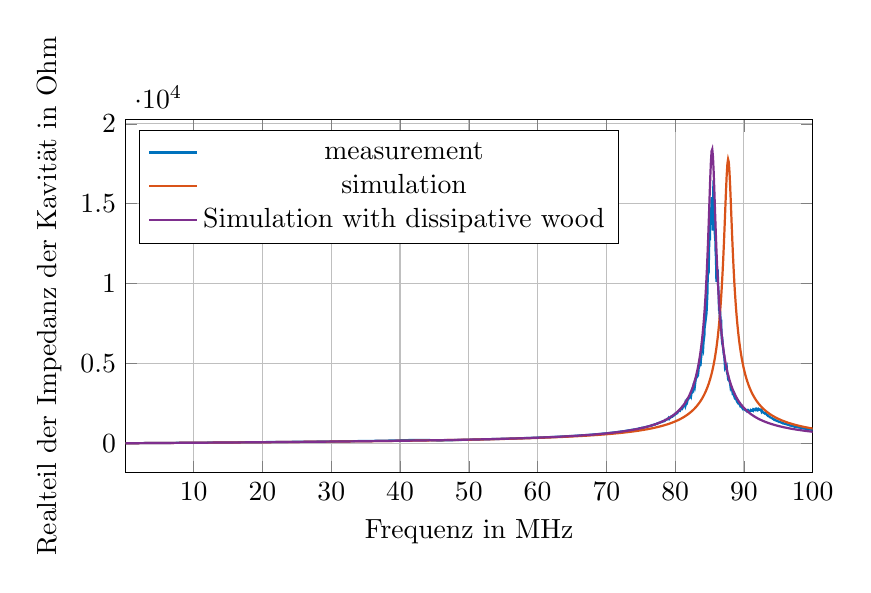
\begin{tikzpicture}

\begin{axis}[%
width=0.85\textwidth, height = 0.5\textwidth, xmin = 0.1, xmax = 100, xlabel=Frequenz in MHz, ylabel=Realteil der Impedanz der Kavit\"at in Ohm, xticklabel style={/pgf/number format/fixed,/pgf/number format/precision=5}, every axis plot/.append style={thick},every axis legend/.append style={at={(0.02,0.97)},anchor=north west}, grid=both, cycle list name=color list]
\addplot [color=mycolor1]
  table[row sep=crcr]{%
0.03	0.155043328782634\\
0.092481	0.328085826583243\\
0.154963	0.534414872921778\\
0.217444	0.741008202451228\\
0.279925	0.936915162072986\\
0.342406	1.14613904443054\\
0.404888	1.3395822292883\\
0.467369	1.53325399164652\\
0.52985	1.78224567823855\\
0.592331	1.93842741832136\\
0.654813	2.18014690534835\\
0.717294	2.3648090481263\\
0.779775	2.56105782521598\\
0.842256	2.76092976411933\\
0.904738	2.99270359701725\\
0.967219	3.1688027175102\\
1.0297	3.38138810817392\\
1.092181	3.62143165949601\\
1.154663	3.77822327032165\\
1.217144	3.99554366668667\\
1.279625	4.1943222764709\\
1.342106	4.40630327223399\\
1.404588	4.60143617254439\\
1.467069	4.82063665919762\\
1.52955	5.03698521935493\\
1.592031	5.22763385638283\\
1.654513	5.43417003949085\\
1.716994	5.64894963266624\\
1.779475	5.85720317643156\\
1.841956	6.04932145137783\\
1.904438	6.26546074667298\\
1.966919	6.4569791582442\\
2.0294	6.71000641716534\\
2.091881	6.88332842005959\\
2.154363	7.10067992350733\\
2.216844	7.3379025383765\\
2.279325	7.51272603908861\\
2.341806	7.68041216530077\\
2.404288	7.93858112902425\\
2.466769	8.12842838132932\\
2.52925	8.31207027595412\\
2.591731	8.53525198714719\\
2.654213	8.73753060082767\\
2.716694	8.91752032639119\\
2.779175	9.14842190546545\\
2.841656	9.36148334817191\\
2.904138	9.55220011231125\\
2.966619	9.79602708579351\\
3.0291	9.97561817039927\\
3.091581	10.0518454692111\\
3.154063	10.4981608280736\\
3.216544	10.6240339541814\\
3.279025	10.7007131599534\\
3.341506	11.0060515633946\\
3.403988	11.1850825397446\\
3.466469	11.4010230989372\\
3.52895	11.6330226382699\\
3.591431	11.8291729162102\\
3.653913	12.04503102842\\
3.716394	12.1870113054842\\
3.778875	12.4590582247656\\
3.841356	12.648154420705\\
3.903838	12.8800520582954\\
3.966319	13.0601025684181\\
4.0288	13.2770589063429\\
4.091281	13.4830732040177\\
4.153763	13.7130922145262\\
4.216244	13.8660445775138\\
4.278725	14.0750796789787\\
4.341206	14.2961064920628\\
4.403688	14.5101564452076\\
4.466169	14.7201089700314\\
4.52865	14.8990450037712\\
4.591131	15.1290375112265\\
4.653613	15.3411045589814\\
4.716094	15.5470677560111\\
4.778575	15.7510460556783\\
4.841056	15.9530618699013\\
4.903538	16.1710106969231\\
4.966019	16.3550820309774\\
5.0285	16.5830083085066\\
5.090981	16.7800954574162\\
5.153463	16.9790620415263\\
5.215944	17.1900134453118\\
5.278425	17.4211459063404\\
5.340906	17.5910211838313\\
5.403388	17.8140809386844\\
5.465869	18.0180985722689\\
5.52835	18.2391140478369\\
5.590831	18.4740454963173\\
5.653313	18.6470858999469\\
5.715794	18.8611539265232\\
5.778275	19.1001022575797\\
5.840756	19.2920570082612\\
5.903238	19.4781097943307\\
5.965719	19.7020087798174\\
6.0282	19.9382487736511\\
6.090681	20.1091965083143\\
6.153163	20.3420517846652\\
6.215644	20.5340628381234\\
6.278125	20.7400179674464\\
6.340606	20.914008271013\\
6.403088	21.2100175692997\\
6.465569	21.3930972336873\\
6.52805	21.6061143681598\\
6.590531	21.7710955454704\\
6.653013	21.9372441580523\\
6.715494	22.1950167895859\\
6.777975	22.45507387563\\
6.840456	22.602083670538\\
6.902938	22.8270995038792\\
6.965419	23.0252326209748\\
7.0279	23.2610713158272\\
7.090381	23.3181148946479\\
7.152863	23.6570194041853\\
7.215344	23.8861407514902\\
7.277825	24.1240493582649\\
7.340306	24.2650857251731\\
7.402788	24.4810377639511\\
7.465269	24.7690997634149\\
7.52775	24.9481347599375\\
7.590231	25.1311155231916\\
7.652713	25.3540745887126\\
7.715194	25.531081474352\\
7.777675	25.7900958138972\\
7.840156	25.9951293322422\\
7.902638	26.2152043144813\\
7.965119	26.4401271555187\\
8.0276	26.5871007678536\\
8.090081	26.8220921273863\\
8.152563	27.0420769219008\\
8.215044	27.18802531281\\
8.277525	27.4260828183684\\
8.340006	27.6740599435645\\
8.402488	27.8110679990899\\
8.464969	28.1090953116602\\
8.52745	28.3090473919558\\
8.589931	28.524072925338\\
8.652413	28.7321170121521\\
8.714894	28.9250573510235\\
8.777375	29.1350649089718\\
8.839856	29.395084063326\\
8.902338	29.5781424575648\\
8.964819	29.7550557512501\\
9.0273	29.9890553162316\\
9.089781	30.2001874325309\\
9.152263	30.3740304372008\\
9.214744	30.6641845963658\\
9.277225	30.8480868489441\\
9.339706	31.1040607999984\\
9.402188	31.3052050287169\\
9.464669	31.4762039148624\\
9.52715	31.6980291658646\\
9.589631	31.8880774912819\\
9.652113	32.1230370675003\\
9.714594	32.3670311429702\\
9.777075	32.5780844992458\\
9.839556	32.7730634706309\\
9.902038	33.0682590834474\\
9.964519	33.2030097153857\\
10.027	33.424172551613\\
10.089481	33.6521307265974\\
10.151963	33.811114258628\\
10.214444	34.018113563365\\
10.276925	34.2930802734313\\
10.339406	34.5182263304475\\
10.401888	34.6861214787701\\
10.464369	34.9080963101685\\
10.52685	35.1111828039159\\
10.589331	35.3551514952206\\
10.651813	35.55910864195\\
10.714294	35.7640511722316\\
10.776775	36.0081221731987\\
10.839256	36.2151832252717\\
10.901738	36.4360326797526\\
10.964219	36.6371633366995\\
11.0267	36.8752118637981\\
11.089181	37.072128739661\\
11.151663	37.2620558242564\\
11.214144	37.5252015850681\\
11.276625	37.7271265045458\\
11.339106	37.9491576897301\\
11.401588	38.1781011891634\\
11.464069	38.3952034764761\\
11.52655	38.5901550704321\\
11.589031	38.8442762611173\\
11.651513	39.0230822079702\\
11.713994	39.2830816638664\\
11.776475	39.4802718107411\\
11.838956	39.7092560464182\\
11.901438	39.9202905211122\\
11.963919	40.1623678785253\\
12.0264	40.3591327118163\\
12.088881	40.5371866068675\\
12.151363	40.7481856405902\\
12.213844	41.0413847023952\\
12.276325	41.1681159307783\\
12.338806	41.443024322677\\
12.401288	41.6451994857751\\
12.463769	41.9121376066647\\
12.52625	42.1932214448008\\
12.588731	42.3281845700947\\
12.651213	42.5684480112912\\
12.713694	42.7421769801212\\
12.776175	42.9693133504598\\
12.838656	43.258074159745\\
12.901138	43.408152863719\\
12.963619	43.6782327797268\\
13.0261	43.8592130331815\\
13.088581	44.1092564113248\\
13.151063	44.2971934078221\\
13.213544	44.5101490790584\\
13.276025	44.7480716904092\\
13.338506	45.0140977299335\\
13.400988	45.268183520106\\
13.463469	45.4144033315423\\
13.52595	45.6392227777818\\
13.588431	45.8894846322118\\
13.650913	46.1212025850367\\
13.713394	46.4022437405779\\
13.775875	46.5333245689581\\
13.838356	46.8322476429436\\
13.900838	47.0703891417949\\
13.963319	47.2114800383339\\
14.0258	47.4733325804077\\
14.088281	47.6624930762124\\
14.150763	47.8854907799847\\
14.213244	48.1212112873315\\
14.275725	48.3734348068235\\
14.338206	48.6335931742659\\
14.400688	48.8556098090076\\
14.463169	49.1055316359573\\
14.52565	49.3139290291293\\
14.588131	49.5240357916234\\
14.650613	49.7718969142226\\
14.713094	49.937143214345\\
14.775575	50.0989622073152\\
14.838056	50.3309577720313\\
14.900538	50.5258835295337\\
14.963019	50.7758116765257\\
15.0255	51.0260299321827\\
15.087981	51.2962590581419\\
15.150463	51.4665273478792\\
15.212944	51.7288670787405\\
15.275425	51.9175140800289\\
15.337906	52.0410066197801\\
15.400388	52.2729977139249\\
15.462869	52.5285405688184\\
15.52535	52.7841066632751\\
15.587831	52.9805274255551\\
15.650313	53.1383932768013\\
15.712794	53.3209506531907\\
15.775275	53.5910899986182\\
15.837756	53.7978960485445\\
15.900238	54.1079368259408\\
15.962719	54.3148546724559\\
16.0252	54.4758848964384\\
16.087681	54.8229585998421\\
16.150163	54.9328126481796\\
16.212644	55.1879522598909\\
16.275125	55.3838381758614\\
16.337606	55.7015097451586\\
16.400088	55.8226793441519\\
16.462569	56.1355307252902\\
16.52505	56.3965541145911\\
16.587531	56.5805786892464\\
16.650013	56.8245242902217\\
16.712494	57.0085225980292\\
16.774975	57.3425709993021\\
16.837456	57.4887168965354\\
16.899938	57.7525158656313\\
16.962419	57.9715390601285\\
17.0249	58.1868284601421\\
17.087381	58.3874862953527\\
17.149863	58.6684376096722\\
17.212344	58.9245811431019\\
17.274825	59.1195792262597\\
17.337306	59.3697230076072\\
17.399788	59.5644533741392\\
17.462269	59.809522494332\\
17.52475	60.064570113254\\
17.587231	60.2665432956794\\
17.649713	60.5785652759291\\
17.712194	60.6995641490942\\
17.774675	61.0847308043508\\
17.837156	61.2622930867757\\
17.899638	61.4372743370016\\
17.962119	61.707506423449\\
18.0246	62.0295037945654\\
18.087081	62.1896362000133\\
18.149563	62.3914328314393\\
18.212044	62.6236581126494\\
18.274525	62.9166550478488\\
18.337006	63.1115425884204\\
18.399488	63.3617607966351\\
18.461969	63.5744915512503\\
18.52445	63.7815368887423\\
18.586931	64.0822976030822\\
18.649413	64.2814861449236\\
18.711894	64.4884402888611\\
18.774375	64.7585287888012\\
18.836856	64.9491975704088\\
18.899338	65.2462063633588\\
18.961819	65.4655708946313\\
19.0243	65.7425208741649\\
19.086781	65.9847399953201\\
19.149263	66.246755580632\\
19.211744	66.4965149680041\\
19.274225	66.7342315580242\\
19.336706	66.9373446443762\\
19.399188	67.3052295935465\\
19.461669	67.4063941050847\\
19.52415	67.687259696711\\
19.586631	67.9772479434112\\
19.649113	68.1094168811479\\
19.711594	68.3832788851924\\
19.774075	68.6523869523122\\
19.836556	68.9654531269098\\
19.899038	69.1411855918019\\
19.961519	69.4224932632789\\
20.024	69.7194482264454\\
20.086481	69.9413670767165\\
20.148963	70.1683658891954\\
20.211444	70.4617638908508\\
20.273925	70.6845137653928\\
20.336406	70.9104004141141\\
20.398888	71.1456033356946\\
20.461369	71.363554414631\\
20.52385	71.6338250230992\\
20.586331	71.8530616770086\\
20.648813	72.0476947442456\\
20.711294	72.3407798465706\\
20.773775	72.613560083775\\
20.836256	72.8206374737958\\
20.898738	73.1253882853965\\
20.961219	73.3327339842856\\
21.0237	73.5705080012365\\
21.086181	73.8595811658853\\
21.148663	74.0907614268473\\
21.211144	74.2936089420887\\
21.273625	74.5746712024934\\
21.336106	74.8167899233855\\
21.398588	75.0559563939465\\
21.461069	75.3555696282631\\
21.52355	75.6216456925529\\
21.586031	75.7895220376141\\
21.648513	76.1178301664597\\
21.710994	76.4346548691103\\
21.773475	76.539653970736\\
21.835956	76.8365586488619\\
21.898438	77.1177315395753\\
21.960919	77.4656303224211\\
22.0234	77.6455978603423\\
22.085881	77.9184796538023\\
22.148363	78.1915489679032\\
22.210844	78.438805601883\\
22.273325	78.6058216251188\\
22.335806	78.887666175645\\
22.398288	79.177062587848\\
22.460769	79.3719611031503\\
22.52325	79.680793044811\\
22.585731	79.9070729961372\\
22.648213	80.1458591582248\\
22.710694	80.3407523943484\\
22.773175	80.7202716832024\\
22.835656	80.9266493909145\\
22.898138	81.172601536787\\
22.960619	81.4270332263186\\
23.0231	81.7276585900392\\
23.085581	82.0132516341719\\
23.148063	82.262718423597\\
23.210544	82.4968701297813\\
23.273025	82.7777302436471\\
23.335506	83.0871314040869\\
23.397988	83.2387758941709\\
23.460469	83.5481251612506\\
23.52295	83.8023775393634\\
23.585431	84.0712421045389\\
23.647913	84.3100169600861\\
23.710394	84.5518143874512\\
23.772875	84.841148235747\\
23.835356	85.0910653690504\\
23.897838	85.4420034866341\\
23.960319	85.7350573665172\\
24.0228	85.8839240577653\\
24.085281	86.2001301330804\\
24.147763	86.4498824138009\\
24.210244	86.7201233564621\\
24.272725	87.0630412381741\\
24.335206	87.2596653260256\\
24.397688	87.5992331190177\\
24.460169	87.7942936446327\\
24.52265	88.0522898541543\\
24.585131	88.415221738341\\
24.647613	88.6489671841133\\
24.710094	88.8212161537996\\
24.772575	89.149402151669\\
24.835056	89.3216268817916\\
24.897538	89.6037656030705\\
24.960019	89.9788321475668\\
25.0225	90.2474506725259\\
25.084981	90.540747330967\\
25.147463	90.7987423660152\\
25.209944	91.149307956177\\
25.272425	91.1893707840996\\
25.334906	91.6144290267095\\
25.397388	91.8500216241673\\
25.459869	92.0455385011137\\
25.52235	92.2990117897261\\
25.584831	92.6774126359276\\
25.647313	92.9929220038278\\
25.709794	93.1776279835455\\
25.772275	93.5103305952877\\
25.834756	93.7865494290626\\
25.897238	93.9978260110839\\
25.959719	94.3262285822984\\
26.0222	94.5093226300982\\
26.084681	94.8762565760791\\
26.147163	94.9361350745331\\
26.209644	95.3763726605809\\
26.272125	95.7163677846689\\
26.334606	96.0103510753398\\
26.397088	96.2048567084323\\
26.459569	96.4385729344851\\
26.52205	96.8149179484236\\
26.584531	97.1701633556309\\
26.647013	97.4161578926207\\
26.709494	97.6705588854697\\
26.771975	97.9756367799669\\
26.834456	98.1981082032134\\
26.896938	98.6489153017406\\
26.959419	98.8557018297377\\
27.0219	98.9651133798673\\
27.084381	99.369889553325\\
27.146863	99.5776749891762\\
27.209344	99.7612455119221\\
27.271825	100.052781896407\\
27.334306	100.403745128556\\
27.396788	100.543944463901\\
27.459269	100.953825906748\\
27.52175	101.143201165921\\
27.584231	101.502223865342\\
27.646713	101.603004038709\\
27.709194	102.072448530443\\
27.771675	102.202286221787\\
27.834156	102.56279959537\\
27.896638	102.843365483632\\
27.959119	103.112784662427\\
28.0216	103.391960455782\\
28.084081	103.821148312326\\
28.146563	104.053326347599\\
28.209044	104.322395721149\\
28.271525	104.532084854556\\
28.334006	104.872463370706\\
28.396488	105.242987647634\\
28.458969	105.462140361411\\
28.52145	105.791622441524\\
28.583931	106.092202394709\\
28.646413	106.271427395326\\
28.708894	106.652609744019\\
28.771375	106.871804818717\\
28.833856	107.301889018274\\
28.896338	107.481885854734\\
28.958819	107.882240624164\\
29.0213	108.161462666931\\
29.083781	108.401399348163\\
29.146263	108.681260332957\\
29.208744	109.342466331065\\
29.271225	109.471385670594\\
29.333706	109.771563616494\\
29.396188	110.11143676408\\
29.458669	110.522439999124\\
29.52115	110.731613125114\\
29.583631	110.991609346338\\
29.646113	111.341732361276\\
29.708594	111.752236438471\\
29.771075	111.803095771092\\
29.833556	112.101411258958\\
29.896038	112.571464437663\\
29.958519	112.901520267931\\
30.021	113.172135890819\\
30.083481	113.663308221431\\
30.145963	113.902520871313\\
30.208444	114.261327581295\\
30.270925	114.391623243837\\
30.333406	114.922033174496\\
30.395888	115.222027880783\\
30.458369	115.39188864058\\
30.52085	115.683338753729\\
30.583331	116.151809811815\\
30.645813	116.46187128859\\
30.708294	116.502217461472\\
30.770775	116.911119817107\\
30.833256	117.322680028203\\
30.895738	117.683459098082\\
30.958219	117.961718311027\\
31.0207	118.16258303579\\
31.083181	118.74190098533\\
31.145663	118.911964952901\\
31.208144	119.30202614411\\
31.270625	119.661952637252\\
31.333106	119.912321156794\\
31.395588	120.352146526101\\
31.458069	120.612763043386\\
31.52055	120.931272184204\\
31.583031	121.412364942126\\
31.645513	121.641987167631\\
31.707994	121.943000948189\\
31.770475	122.322111956261\\
31.832956	122.573151078081\\
31.895438	122.912217402868\\
31.957919	123.312833187832\\
32.0204	123.681782930268\\
32.082881	124.143510539053\\
32.145363	124.371987399133\\
32.207844	124.572964435948\\
32.270325	124.942849328963\\
32.332806	125.462555691489\\
32.395288	125.71237905457\\
32.457769	125.973316534931\\
32.52025	126.502485544751\\
32.582731	126.792528883369\\
32.645213	126.952261739758\\
32.707694	127.38342124845\\
32.770175	127.713078174829\\
32.832656	128.242621620115\\
32.895138	128.67370916003\\
32.957619	128.983753457558\\
33.0201	129.453567046258\\
33.082581	129.383285180119\\
33.145063	129.873674888331\\
33.207544	130.313318582561\\
33.270025	130.703474357035\\
33.332506	131.092973835366\\
33.394988	131.444619532334\\
33.457469	131.82379299656\\
33.51995	132.183435456187\\
33.582431	132.685599674569\\
33.644913	132.843885278924\\
33.707394	133.333132776516\\
33.769875	133.634039155449\\
33.832356	134.054915627887\\
33.894838	134.404323159637\\
33.957319	134.874372272867\\
34.0198	135.204178814858\\
34.082281	135.736653988523\\
34.144763	136.043337980954\\
34.207244	136.174266967001\\
34.269725	136.76365599091\\
34.332206	136.985423899771\\
34.394688	137.635531953053\\
34.457169	137.566410086183\\
34.51965	138.246917828211\\
34.582131	138.606741138373\\
34.644613	138.994064869691\\
34.707094	139.226257580961\\
34.769575	139.895656344291\\
34.832056	140.306069095389\\
34.894538	140.656642889698\\
34.957019	140.896183411759\\
35.0195	141.23580941461\\
35.081981	141.637299974265\\
35.144463	142.167589699622\\
35.206944	142.647886770187\\
35.269425	142.715003153137\\
35.331906	143.14869780756\\
35.394388	143.647831866687\\
35.456869	144.126635598698\\
35.51935	144.778941082604\\
35.581831	144.926820278374\\
35.644313	145.189353273579\\
35.706794	145.848120046163\\
35.769275	146.009132210968\\
35.831756	146.599799198362\\
35.894238	147.039689349509\\
35.956719	147.377401351089\\
36.0192	147.84809369417\\
36.081681	148.017835509779\\
36.144163	148.688705963163\\
36.206644	148.948615314141\\
36.269125	149.742130798249\\
36.331606	149.988555576751\\
36.394088	150.272088013709\\
36.456569	150.942135588443\\
36.51905	151.365584212528\\
36.581531	151.645213587505\\
36.644013	152.504486832355\\
36.706494	152.714466911292\\
36.768975	153.183892328795\\
36.831456	153.543235461547\\
36.893938	154.352559295271\\
36.956419	154.282667299344\\
37.0189	154.933935869454\\
37.081381	155.39628985275\\
37.143863	155.915677598502\\
37.206344	156.536286413087\\
37.268825	156.997844217683\\
37.331306	157.396413329529\\
37.393788	157.900046409113\\
37.456269	158.369986916713\\
37.51875	158.869671429131\\
37.581231	159.084502086155\\
37.643713	159.914044502039\\
37.706194	160.218779202065\\
37.768675	160.636287731011\\
37.831156	161.290989531344\\
37.893638	161.727678719507\\
37.956119	162.226173584906\\
38.0186	163.083492496942\\
38.081081	163.260817356768\\
38.143563	163.523402377152\\
38.206044	164.460901870323\\
38.268525	164.698027070758\\
38.331006	165.440718820972\\
38.393488	165.872769944316\\
38.455969	166.505332647336\\
38.51845	167.117816001167\\
38.580931	167.378418549107\\
38.643413	167.992038692314\\
38.705894	168.760984839506\\
38.768375	168.882151599866\\
38.830856	169.787857519317\\
38.893338	170.775042040692\\
38.955819	170.930921673055\\
39.0183	171.557801364438\\
39.080781	172.396752025669\\
39.143263	172.647230284763\\
39.205744	173.378101215234\\
39.268225	173.843626886349\\
39.330706	174.660242496683\\
39.393188	175.137302734169\\
39.455669	175.92237574851\\
39.51815	176.306789741632\\
39.580631	177.294014363148\\
39.643113	177.83256850476\\
39.705594	178.116916728872\\
39.768075	178.768484719763\\
39.830556	179.637926017865\\
39.893038	180.348293202348\\
39.955519	180.832530491613\\
40.018	181.472674097232\\
40.080481	182.309556219634\\
40.142963	182.708217943255\\
40.205444	184.237696416884\\
40.267925	184.859810464579\\
40.330406	185.089574598355\\
40.392888	186.009986011504\\
40.455369	186.564561278395\\
40.51785	187.415780562897\\
40.580331	188.080041272326\\
40.642813	189.154744918017\\
40.705294	189.756963036933\\
40.767775	190.657587312963\\
40.830256	191.356892836396\\
40.892738	192.395594169929\\
40.955219	193.401634677683\\
41.0177	193.789264264045\\
41.080181	194.837541772627\\
41.142663	195.844033120746\\
41.205144	196.511441997661\\
41.267625	197.300986981819\\
41.330106	197.296012075764\\
41.392588	198.490733992799\\
41.455069	198.94414010219\\
41.51755	199.628855441792\\
41.580031	200.290802647051\\
41.642513	200.74474907454\\
41.704994	200.950517381767\\
41.767475	201.262764874678\\
41.829956	201.727983752875\\
41.892438	201.300504211987\\
41.954919	201.389497911386\\
42.0174	201.692149663788\\
42.079881	201.558652763904\\
42.142363	201.306148033288\\
42.204844	201.72525035057\\
42.267325	201.593543500282\\
42.329806	201.62216668809\\
42.392288	201.64593438996\\
42.454769	202.342067699725\\
42.51725	201.851406148186\\
42.579731	202.281395229517\\
42.642213	202.395927488673\\
42.704694	202.279081036572\\
42.767175	202.205142031552\\
42.829656	202.648641448691\\
42.892138	203.22688035789\\
42.954619	203.477760445706\\
43.0171	204.15124505131\\
43.079581	204.922217255719\\
43.142063	205.244297998751\\
43.204544	205.182536186684\\
43.267025	206.175512124985\\
43.329506	206.03269957946\\
43.391988	205.76487553516\\
43.454469	206.529604224189\\
43.51695	205.936265094325\\
43.579431	205.831680982302\\
43.641913	205.904669456523\\
43.704394	206.00821849868\\
43.766875	205.14896277827\\
43.829356	205.430124772391\\
43.891838	205.400864849689\\
43.954319	204.456259977532\\
44.0168	203.90486968437\\
44.079281	202.399175791306\\
44.141763	200.955591870443\\
44.204244	200.534693479707\\
44.266725	198.855839582347\\
44.329206	197.418978317689\\
44.391688	196.478009202048\\
44.454169	195.082141368707\\
44.51665	194.360972700283\\
44.579131	193.052924891077\\
44.641613	191.663457813429\\
44.704094	190.210863046778\\
44.766575	188.808493212037\\
44.829056	186.976556701636\\
44.891538	185.592865821938\\
44.954019	184.231037439406\\
45.0165	182.887164724592\\
45.078981	181.682356108126\\
45.141463	180.695231414667\\
45.203944	180.226307180722\\
45.266425	178.984249016499\\
45.328906	178.230223306823\\
45.391388	177.744770567238\\
45.453869	177.46472353682\\
45.51635	177.069761622362\\
45.578831	176.890340041507\\
45.641313	176.682601022285\\
45.703794	176.042916247715\\
45.766275	176.837631812349\\
45.828756	176.558338109532\\
45.891238	176.978517521195\\
45.953719	177.010161745025\\
46.0162	177.406167336426\\
46.078681	177.361204878632\\
46.141163	177.683717610815\\
46.203644	178.233377906609\\
46.266125	178.449667929083\\
46.328606	178.988172503101\\
46.391088	179.485382471665\\
46.453569	180.025623887268\\
46.51605	180.660056736402\\
46.578531	181.630016693277\\
46.641013	181.714748438315\\
46.703494	182.557349950639\\
46.765975	183.019850027258\\
46.828456	183.887748379276\\
46.890938	184.527573714608\\
46.953419	185.196069907004\\
47.0159	186.033237914626\\
47.078381	186.510278861515\\
47.140863	187.582117647179\\
47.203344	188.000321608767\\
47.265825	189.102780741056\\
47.328306	189.618841363405\\
47.390788	190.462849805415\\
47.453269	191.185023014356\\
47.51575	192.092757281476\\
47.578231	192.941437801733\\
47.640713	193.310359600824\\
47.703194	194.207873383136\\
47.765675	194.999592963678\\
47.828156	195.904591015627\\
47.890638	196.719353702171\\
47.953119	197.21165874258\\
48.0156	198.818337272999\\
48.078081	199.361972261512\\
48.140563	200.001064957165\\
48.203044	200.925386103897\\
48.265525	201.812138210267\\
48.328006	202.226023903948\\
48.390488	202.845902980563\\
48.452969	203.926490883357\\
48.51545	204.926769381162\\
48.577931	205.578441051099\\
48.640413	206.285209028665\\
48.702894	207.238713333199\\
48.765375	207.881046909044\\
48.827856	208.21137185322\\
48.890338	209.083828126424\\
48.952819	210.054934719468\\
49.0153	210.605657628184\\
49.077781	211.503421629533\\
49.140263	212.471459563396\\
49.202744	213.473588082929\\
49.265225	213.324566754511\\
49.327706	214.378294572935\\
49.390188	215.22372425223\\
49.452669	215.730089391814\\
49.51515	217.231064723718\\
49.577631	217.915270589282\\
49.640113	217.98426438851\\
49.702594	218.912541312735\\
49.765075	219.869863512488\\
49.827556	220.125530143598\\
49.890038	221.047124468969\\
49.952519	222.07122947604\\
50.015	222.798522876612\\
50.077481	223.803587703593\\
50.139963	224.252022575048\\
50.202444	225.369613222369\\
50.264925	225.274259250807\\
50.327406	225.453162089158\\
50.389888	226.874615109315\\
50.452369	227.176166188269\\
50.51485	227.626709603684\\
50.577331	228.773294848853\\
50.639813	229.712721077872\\
50.702294	230.073190519887\\
50.764775	231.257344586069\\
50.827256	231.182584344063\\
50.889738	232.587900149599\\
50.952219	233.414185749281\\
51.0147	233.930497789408\\
51.077181	234.271777278015\\
51.139663	234.878526766497\\
51.202144	235.792407426533\\
51.264625	236.543912413742\\
51.327106	237.56211419332\\
51.389588	237.887534847877\\
51.452069	238.707283919029\\
51.51455	239.088641263026\\
51.577031	240.2528977973\\
51.639513	240.944029259909\\
51.701994	241.164112786293\\
51.764475	241.818068315831\\
51.826956	243.042936132692\\
51.889438	243.397303660086\\
51.951919	243.77153491743\\
52.0144	244.088862763134\\
52.076881	245.531672091402\\
52.139363	245.67827405776\\
52.201844	246.532295501015\\
52.264325	247.063397240465\\
52.326806	248.141024911239\\
52.389288	248.419456180469\\
52.451769	249.310644177099\\
52.51425	250.51127775212\\
52.576731	250.613794001847\\
52.639213	251.245486725633\\
52.701694	251.655791024169\\
52.764175	252.766417826815\\
52.826656	253.905558537028\\
52.889138	254.574291317878\\
52.951619	254.929730374862\\
53.0141	255.655678567874\\
53.076581	256.614539424406\\
53.139063	257.52876598353\\
53.201544	257.592865941586\\
53.264025	258.651605253089\\
53.326506	259.814151002212\\
53.388988	259.857554789158\\
53.451469	260.954177895277\\
53.51395	261.794508118486\\
53.576431	262.986137193579\\
53.638913	263.098409081089\\
53.701394	264.362274131541\\
53.763875	264.3479834158\\
53.826356	265.472643564266\\
53.888838	266.550130339492\\
53.951319	266.465830725067\\
54.0138	268.145662886797\\
54.076281	268.275725441196\\
54.138763	269.068479677572\\
54.201244	270.693486438074\\
54.263725	270.984357364037\\
54.326206	271.22989262985\\
54.388688	271.707328491522\\
54.451169	273.292207141001\\
54.51365	274.155552115948\\
54.576131	274.38074592799\\
54.638613	275.697904527764\\
54.701094	276.213712288148\\
54.763575	276.881428116802\\
54.826056	278.393665712782\\
54.888538	280.059252987649\\
54.951019	279.603060650273\\
55.0135	280.635853676967\\
55.075981	280.764937670287\\
55.138463	281.645948815175\\
55.200944	283.459368991395\\
55.263425	283.47965474792\\
55.325906	283.873691074041\\
55.388388	285.054481957397\\
55.450869	284.422936234053\\
55.51335	286.958617399792\\
55.575831	287.088563687236\\
55.638313	288.24616906561\\
55.700794	288.556633671798\\
55.763275	289.723584316155\\
55.825756	290.879775584347\\
55.888238	291.613212363569\\
55.950719	293.340925347964\\
56.0132	291.961627026567\\
56.075681	294.519532214758\\
56.138163	294.586740721642\\
56.200644	295.969843659789\\
56.263125	295.904824624405\\
56.325606	297.664672255543\\
56.388088	298.602842812991\\
56.450569	299.275839078266\\
56.51305	300.211685783548\\
56.575531	300.488726592197\\
56.638013	301.547440970737\\
56.700494	303.712948326211\\
56.762975	303.995127541545\\
56.825456	304.056219202962\\
56.887938	305.831342914686\\
56.950419	306.995168497812\\
57.0129	307.022410185315\\
57.075381	308.047053944686\\
57.137863	308.95227256811\\
57.200344	310.357185893931\\
57.262825	311.037506072821\\
57.325306	311.385583873114\\
57.387788	312.373022612389\\
57.450269	312.855381735715\\
57.51275	314.038977969296\\
57.575231	315.680123652092\\
57.637713	316.365505761927\\
57.700194	317.568328050831\\
57.762675	318.877485495605\\
57.825156	319.938295357089\\
57.887638	320.456719825002\\
57.950119	320.473521683149\\
58.0126	321.56335368944\\
58.075081	322.9239496863\\
58.137563	322.432710034202\\
58.200044	324.332007979478\\
58.262525	325.170700372896\\
58.325006	325.499949015357\\
58.387488	327.694344998506\\
58.449969	328.975126998988\\
58.51245	329.180986481601\\
58.574931	329.962052903057\\
58.637413	332.485147391579\\
58.699894	332.401389078024\\
58.762375	333.619233745598\\
58.824856	335.156375605478\\
58.887338	335.225957838888\\
58.949819	336.815752762545\\
59.0123	337.430874492836\\
59.074781	339.057963563754\\
59.137263	337.954772093841\\
59.199744	340.739070527581\\
59.262225	341.4890730082\\
59.324706	342.330216762996\\
59.387188	342.604773330729\\
59.449669	345.057874108098\\
59.51215	345.492690018183\\
59.574631	345.968597540297\\
59.637113	346.580844969828\\
59.699594	348.703877030354\\
59.762075	350.259209170865\\
59.824556	350.466397905705\\
59.887038	352.645891063543\\
59.949519	353.795944099137\\
60.012	354.302761588165\\
60.074481	354.904845851673\\
60.136963	357.196914713719\\
60.199444	357.577491159609\\
60.261925	358.896365125087\\
60.324406	359.652404564463\\
60.386888	359.028429321412\\
60.449369	363.716336972922\\
60.51185	363.813980077731\\
60.574331	363.428057701934\\
60.636813	364.358683937957\\
60.699294	366.666332984091\\
60.761775	367.285239540061\\
60.824256	368.708772388182\\
60.886738	369.689775806689\\
60.949219	370.963599637485\\
61.0117	373.520256560471\\
61.074181	373.444744321031\\
61.136663	374.629633586293\\
61.199144	375.858149850446\\
61.261625	375.775313932408\\
61.324106	378.543981963787\\
61.386588	380.456698240417\\
61.449069	379.220159512914\\
61.51155	381.905367513996\\
61.574031	383.880765161528\\
61.636513	384.089682966101\\
61.698994	383.708594458086\\
61.761475	384.631889043277\\
61.823956	386.93740238054\\
61.886438	388.028962300496\\
61.948919	390.316016915781\\
62.0114	390.218499408985\\
62.073881	393.650998454215\\
62.136363	394.688943164107\\
62.198844	393.762446438205\\
62.261325	396.325027573329\\
62.323806	397.479094772291\\
62.386288	397.828650858633\\
62.448769	399.306004507821\\
62.51125	400.833482958946\\
62.573731	403.205529049392\\
62.636213	403.959973863748\\
62.698694	403.999818719019\\
62.761175	405.693379636641\\
62.823656	407.98929339506\\
62.886138	408.269321840375\\
62.948619	410.751057066199\\
63.0111	411.140599504598\\
63.073581	411.643994835343\\
63.136063	412.918200233412\\
63.198544	413.822194590865\\
63.261025	416.840986138599\\
63.323506	415.912146109007\\
63.385988	418.474555063985\\
63.448469	420.277263968681\\
63.51095	422.191431087842\\
63.573431	423.671363138931\\
63.635913	424.69671122461\\
63.698394	426.639244744316\\
63.760875	428.196825099159\\
63.823356	428.620584294548\\
63.885838	430.222125981452\\
63.948319	433.189606680493\\
64.0108	432.421498685021\\
64.073281	434.761713075105\\
64.135763	435.426572863899\\
64.198244	438.183099213103\\
64.260725	438.574256391093\\
64.323206	438.049987112202\\
64.385688	441.828036779017\\
64.448169	444.316095955346\\
64.51065	444.19809413819\\
64.573131	447.707295081284\\
64.635613	448.555615148222\\
64.698094	452.672291619445\\
64.760575	454.645200058243\\
64.823056	453.040597779051\\
64.885538	452.6470740091\\
64.948019	454.697768062479\\
65.0105	457.208677940391\\
65.072981	459.00551860408\\
65.135463	461.851209872833\\
65.197944	461.258555334207\\
65.260425	462.65985270931\\
65.322906	465.062555604082\\
65.385388	469.437817565862\\
65.447869	470.084675865955\\
65.51035	470.146598478602\\
65.572831	471.856665456789\\
65.635313	474.290675371127\\
65.697794	475.359685749644\\
65.760275	478.698548132329\\
65.822756	477.797152812781\\
65.885238	478.865253339601\\
65.947719	482.948903223726\\
66.0102	484.717887951332\\
66.072681	486.865537889056\\
66.135163	485.892292525823\\
66.197644	491.617700028182\\
66.260125	492.243657588394\\
66.322606	493.185693628678\\
66.385088	495.485245475584\\
66.447569	498.855074506615\\
66.51005	499.36942067872\\
66.572531	501.008761960307\\
66.635013	502.002144976493\\
66.697494	506.358672888102\\
66.759975	505.35088614249\\
66.822456	507.206080093683\\
66.884938	507.780892000674\\
66.947419	511.636341126195\\
67.0099	515.46435557563\\
67.072381	511.819893110848\\
67.134863	517.173052976467\\
67.197344	520.633098699074\\
67.259825	521.745493578047\\
67.322306	521.492700068755\\
67.384788	524.107100539575\\
67.447269	526.099361907996\\
67.50975	527.852933329919\\
67.572231	531.559082733049\\
67.634713	533.204225508388\\
67.697194	534.617262599142\\
67.759675	535.420920338382\\
67.822156	537.637393915267\\
67.884638	538.817128473103\\
67.947119	543.390109814303\\
68.0096	544.433235517451\\
68.072081	549.491838650948\\
68.134563	551.126205814966\\
68.197044	549.324986597187\\
68.259525	553.629042532994\\
68.322006	556.591707650231\\
68.384488	560.50611855358\\
68.446969	561.24320017618\\
68.50945	562.180470077003\\
68.571931	562.785789682895\\
68.634413	565.395830313596\\
68.696894	570.588379131577\\
68.759375	572.873590681225\\
68.821856	575.703405266983\\
68.884338	577.432945111378\\
68.946819	578.662303386872\\
69.0093	579.873039928569\\
69.071781	583.45973677367\\
69.134263	584.223178191348\\
69.196744	588.609514076183\\
69.259225	593.065251836592\\
69.321706	597.663488290861\\
69.384188	598.597917918197\\
69.446669	603.612303159072\\
69.50915	601.350405638011\\
69.571631	605.232052655013\\
69.634113	607.721789858649\\
69.696594	610.777618650192\\
69.759075	609.993034846301\\
69.821556	613.11284977645\\
69.884038	618.617265812231\\
69.946519	619.719824385181\\
70.009	622.612228357266\\
70.071481	624.620540328286\\
70.133963	629.09326648439\\
70.196444	628.474944802098\\
70.258925	632.968969302603\\
70.321406	637.976620524608\\
70.383888	641.854691391284\\
70.446369	643.079790489485\\
70.50885	642.576507584895\\
70.571331	650.867057811348\\
70.633813	650.16888772149\\
70.696294	654.29194792921\\
70.758775	661.331390756555\\
70.821256	661.374475286883\\
70.883738	667.056613685075\\
70.946219	666.120262373094\\
71.0087	669.918893550555\\
71.071181	677.27724563948\\
71.133663	673.971883954368\\
71.196144	680.419649360599\\
71.258625	688.133783772458\\
71.321106	690.484985807077\\
71.383588	687.812130981273\\
71.446069	692.610033113151\\
71.50855	697.608103163947\\
71.571031	705.932515497055\\
71.633513	703.191886378818\\
71.695994	709.48280039829\\
71.758475	714.105774286275\\
71.820956	712.948428402083\\
71.883438	718.361685963972\\
71.945919	721.054039626019\\
72.0084	729.232594971591\\
72.070881	731.377771790338\\
72.133363	732.887892338248\\
72.195844	735.303716547795\\
72.258325	739.52999041621\\
72.320806	741.548831120379\\
72.383288	749.824179348732\\
72.445769	749.304691738281\\
72.50825	756.16741324987\\
72.570731	754.763398585279\\
72.633213	759.234532645216\\
72.695694	765.903818528149\\
72.758175	772.875491100604\\
72.820656	773.802582339966\\
72.883138	781.87857429143\\
72.945619	783.122934758011\\
73.0081	793.097905648477\\
73.070581	794.725232769163\\
73.133063	789.255087241128\\
73.195544	794.220651787021\\
73.258025	808.495779664928\\
73.320506	816.157968509161\\
73.382988	812.035191624107\\
73.445469	815.206979383764\\
73.50795	823.138555302204\\
73.570431	827.418768788816\\
73.632913	829.71050128584\\
73.695394	838.58720599649\\
73.757875	838.918686464904\\
73.820356	844.429054782579\\
73.882838	852.157080846014\\
73.945319	856.024133340293\\
74.0078	857.225338825796\\
74.070281	859.445058416185\\
74.132763	868.105966493147\\
74.195244	865.622675632403\\
74.257725	882.899756448035\\
74.320206	885.722586570423\\
74.382688	886.292030631552\\
74.445169	892.113647040555\\
74.50765	898.050893176996\\
74.570131	898.963079386467\\
74.632613	909.998870806442\\
74.695094	921.739366868965\\
74.757575	931.095052108538\\
74.820056	934.61999043729\\
74.882538	934.678503463089\\
74.945019	938.543056516855\\
75.0075	947.974125451217\\
75.069981	950.883794667361\\
75.132463	957.927943498883\\
75.194944	975.317182738005\\
75.257425	968.454793133887\\
75.319906	970.839763483655\\
75.382388	984.108462803262\\
75.444869	979.847510106037\\
75.50735	982.8126442639\\
75.569831	998.855564664381\\
75.632313	1001.42721114667\\
75.694794	1011.22134908041\\
75.757275	1011.44452904942\\
75.819756	1026.70657171365\\
75.882238	1036.3807649701\\
75.944719	1038.75464672848\\
76.0072	1049.24233311471\\
76.069681	1052.63965197023\\
76.132163	1065.09173013408\\
76.194644	1073.06902709006\\
76.257125	1073.74837019667\\
76.319606	1078.11632772164\\
76.382088	1088.92396887937\\
76.444569	1094.64699647877\\
76.50705	1101.69687464384\\
76.569531	1110.94795382142\\
76.632013	1134.53227036519\\
76.694494	1122.39189791267\\
76.756975	1143.07361250271\\
76.819456	1151.06268556495\\
76.881938	1163.14570884305\\
76.944419	1167.79956007013\\
77.0069	1182.45632735421\\
77.069381	1168.24794718416\\
77.131863	1192.96809550801\\
77.194344	1195.50247431781\\
77.256825	1214.70753521167\\
77.319306	1222.97300710196\\
77.381788	1215.0136608697\\
77.444269	1248.42800997895\\
77.50675	1245.12709234841\\
77.569231	1260.69742349225\\
77.631713	1279.86409184726\\
77.694194	1289.54009898878\\
77.756675	1293.95074233914\\
77.819156	1292.46458922479\\
77.881638	1309.90810597538\\
77.944119	1332.01956577221\\
78.0066	1328.19392669143\\
78.069081	1337.54028350551\\
78.131563	1340.32018044197\\
78.194044	1382.52649652728\\
78.256525	1381.5333607626\\
78.319006	1377.3717642307\\
78.381488	1378.81244351797\\
78.443969	1402.6841291253\\
78.50645	1405.23557316914\\
78.568931	1456.91752206499\\
78.631413	1451.61247104728\\
78.693894	1462.9767109903\\
78.756375	1477.57323121394\\
78.818856	1488.94204386873\\
78.881338	1526.66247170093\\
78.943819	1523.8524590327\\
79.0063	1515.12288399324\\
79.068781	1574.93704115434\\
79.131263	1531.39205381901\\
79.193744	1577.38797145788\\
79.256225	1579.85012773364\\
79.318706	1597.51384873496\\
79.381188	1636.88817654109\\
79.443669	1674.57353451558\\
79.50615	1665.31502007878\\
79.568631	1686.76845657606\\
79.631113	1671.95247839166\\
79.693594	1697.27808375646\\
79.756075	1746.88769244047\\
79.818556	1736.50032064495\\
79.881038	1760.47343734576\\
79.943519	1785.84659265571\\
80.006	1798.09952341354\\
80.068481	1866.54077000745\\
80.130963	1848.91387644206\\
80.193444	1853.84979434689\\
80.255925	1868.08882112174\\
80.318406	1882.79598100803\\
80.380888	1944.44652536397\\
80.443369	1980.61679140615\\
80.50585	2000.67203111854\\
80.568331	2022.1675211515\\
80.630813	2035.85046015173\\
80.693294	2027.02165119172\\
80.755775	2117.2647654226\\
80.818256	2142.88895346912\\
80.880738	2136.83866655861\\
80.943219	2178.80170965602\\
81.0057	2236.87152570281\\
81.068181	2191.75739989626\\
81.130663	2248.51975850781\\
81.193144	2306.03099718976\\
81.255625	2341.4653781126\\
81.318106	2362.63179037699\\
81.380588	2378.2961337899\\
81.443069	2480.45750304253\\
81.50555	2348.55588820024\\
81.568031	2434.41833093657\\
81.630513	2524.53977786051\\
81.692994	2642.9760687528\\
81.755475	2588.67602924738\\
81.817956	2698.39724177149\\
81.880438	2772.1578760958\\
81.942919	2769.72853543447\\
82.0054	2825.58332428899\\
82.067881	2839.84629106929\\
82.130363	2863.59252415563\\
82.192844	3051.81264210305\\
82.255325	3034.19702268986\\
82.317806	2960.97059499077\\
82.380288	3137.8657731012\\
82.442769	3245.650936253\\
82.50525	3224.12581592282\\
82.567731	3282.64767527677\\
82.630213	3471.62464480249\\
82.692694	3387.58296023876\\
82.755175	3534.72216906789\\
82.817656	3714.19653357223\\
82.880138	3608.36008103404\\
82.942619	3835.19225162181\\
83.0051	4007.95175744419\\
83.067581	4069.99614987533\\
83.130063	4132.45336143071\\
83.192544	4147.49789353774\\
83.255025	4204.64857709892\\
83.317506	4238.67674752392\\
83.379988	4461.58688837279\\
83.442469	4825.99781185197\\
83.50495	4790.39986744322\\
83.567431	4876.03354069678\\
83.629913	5332.46292439057\\
83.692394	4839.75948162716\\
83.754875	5255.04369629787\\
83.817356	5471.60628060901\\
83.879838	5779.60755069062\\
83.942319	6076.2789805933\\
84.0048	5978.32783728025\\
84.067281	5881.29029550489\\
84.129763	6322.25816777518\\
84.192244	6540.48946945104\\
84.254725	6739.66742502922\\
84.317206	7530.82246039568\\
84.379688	8226.24835511304\\
84.442169	8164.1814954103\\
84.50465	7927.69449461822\\
84.567131	8144.55985612482\\
84.629613	8738.21825545689\\
84.692094	9318.44001161138\\
84.754575	10648.8884396448\\
84.817056	10611.7957358781\\
84.879538	10702.4805535913\\
84.942019	12252.0636731124\\
85.0045	12911.8714367825\\
85.066981	12719.9703714278\\
85.129463	14296.1081767032\\
85.191944	13669.1538874943\\
85.254425	14588.0775378389\\
85.316906	15408.4558360012\\
85.379388	14632.6821276894\\
85.441869	15121\\
85.50435	13315.4486687456\\
85.566831	16459.8989668831\\
85.629313	15453.5500452161\\
85.691794	13765.896592667\\
85.754275	13270.7831343896\\
85.816756	13372.8239351305\\
85.879238	12064.1492136827\\
85.941719	11580.5010686067\\
86.0042	10105.8890999258\\
86.066681	10751.773365357\\
86.129163	10195.194666116\\
86.191644	10890.647478456\\
86.254125	9840.809889943\\
86.316606	9418.95014213368\\
86.379088	8353.073745634\\
86.441569	8344.28022659834\\
86.50405	7770.59962486808\\
86.566531	8252.66041286081\\
86.629013	7031.52660807026\\
86.691494	7740.35717845113\\
86.753975	6769.70060933274\\
86.816456	6405.5584174996\\
86.878938	6451.17805133295\\
86.941419	6066.03484493784\\
87.0039	5886.22606174788\\
87.066381	5550.28629351676\\
87.128863	5519.17028909237\\
87.191344	5165.84003720595\\
87.253825	4769.45306088654\\
87.316306	4836.7754237715\\
87.378788	4856.27295773209\\
87.441269	4705.29048837582\\
87.50375	4769.62886816155\\
87.566231	4352.55520929948\\
87.628713	4323.71994583368\\
87.691194	4077.54342711393\\
87.753675	4108.04445569909\\
87.816156	3939.81106780516\\
87.878638	3895.76948240011\\
87.941119	3838.67692310775\\
88.0036	3707.43971630019\\
88.066081	3496.52011005228\\
88.128563	3572.39477801656\\
88.191044	3496.46410677988\\
88.253525	3358.67255921145\\
88.316006	3272.83315187316\\
88.378488	3088.78380758512\\
88.440969	3100.15118341025\\
88.50345	3087.01933009821\\
88.565931	2990.31454198384\\
88.628413	3059.36432939916\\
88.690894	2949.53035583633\\
88.753375	2778.06177937065\\
88.815856	2776.60117094623\\
88.878338	2732.18571111116\\
88.940819	2675.93287787642\\
89.0033	2622.08108892536\\
89.065781	2650.06576569337\\
89.128263	2560.82599028126\\
89.190744	2488.84334519069\\
89.253225	2491.97558262516\\
89.315706	2451.65873695749\\
89.378188	2424.14372189439\\
89.440669	2373.80490076586\\
89.50315	2307.48729940167\\
89.565631	2315.86895624515\\
89.628113	2283.7467272883\\
89.690594	2307.42033665303\\
89.753075	2213.78604205555\\
89.815556	2170.66989947804\\
89.878038	2216.24091932714\\
89.940519	2193.38175737832\\
90.003	2167.85475758871\\
90.065481	2111.95631036724\\
90.127963	2090.91976278383\\
90.190444	2080.88761015582\\
90.252925	2057.81562976376\\
90.315406	2070.17607282569\\
90.377888	2068.99351765538\\
90.440369	2017.2002836605\\
90.50285	2058.25462372856\\
90.565331	2028.29544842461\\
90.627813	2060.16206246014\\
90.690294	2024.18828593093\\
90.752775	2004.70149259185\\
90.815256	2018.36389523792\\
90.877738	2010.30918855782\\
90.940219	2027.82707746494\\
91.0027	2078.68653240454\\
91.065181	2056.93160219294\\
91.127663	2030.90814258056\\
91.190144	2035.49035765341\\
91.252625	2032.72897280971\\
91.315106	2093.17478486628\\
91.377588	2052.00344142012\\
91.440069	2105.4028081106\\
91.50255	2080.23664665826\\
91.565031	2082.16108512286\\
91.627513	2120.36057690667\\
91.689994	2095.44246461219\\
91.752475	2171.2590088702\\
91.814956	2176.03273700099\\
91.877438	2128.27269267827\\
91.939919	2089.62995767193\\
92.0024	2132.62641053233\\
92.064881	2150.62158830883\\
92.127363	2087.61045456282\\
92.189844	2104.29390440119\\
92.252325	2121.02397499415\\
92.314806	2100.81908873658\\
92.377288	2096.34396178204\\
92.439769	2106.554581206\\
92.50225	2052.97416128406\\
92.564731	1981.85257867481\\
92.627213	2032.41586957493\\
92.689694	1951.4529213896\\
92.752175	1950.59006100718\\
92.814656	1924.48110328473\\
92.877138	1906.18552349975\\
92.939619	1900.72343135449\\
93.0021	1874.19672222528\\
93.064581	1898.95559305635\\
93.127063	1877.95001863734\\
93.189544	1853.07634384016\\
93.252025	1815.8512081115\\
93.314506	1796.74613955339\\
93.376988	1759.81054764426\\
93.439469	1759.8386444217\\
93.50195	1715.5387036147\\
93.564431	1723.32991908108\\
93.626913	1687.080050294\\
93.689394	1674.82988571974\\
93.751875	1640.1560975712\\
93.814356	1625.11736994594\\
93.876838	1607.15755994862\\
93.939319	1601.70070765421\\
94.0018	1600.96704116606\\
94.064281	1571.30251816765\\
94.126763	1556.20866753145\\
94.189244	1527.96428848975\\
94.251725	1516.01500111312\\
94.314206	1514.45610570264\\
94.376688	1480.47747787665\\
94.439169	1484.87218389328\\
94.50165	1450.05923192813\\
94.564131	1443.69406856162\\
94.626613	1449.15331007454\\
94.689094	1423.07802207047\\
94.751575	1403.13660151106\\
94.814056	1407.85578895709\\
94.876538	1392.59889634453\\
94.939019	1377.0584861944\\
95.0015	1364.05271291105\\
95.063981	1360.48354128229\\
95.126463	1336.35003034385\\
95.188944	1341.41821312371\\
95.251425	1343.25549453557\\
95.313906	1329.33326750668\\
95.376388	1297.94793177539\\
95.438869	1299.92439630157\\
95.50135	1279.29319938785\\
95.563831	1284.50861301122\\
95.626313	1256.17272972311\\
95.688794	1269.56408900851\\
95.751275	1234.76958984257\\
95.813756	1232.50428396821\\
95.876238	1227.49469347122\\
95.938719	1215.23301238898\\
96.0012	1208.8496736981\\
96.063681	1212.32017635606\\
96.126163	1196.35934087547\\
96.188644	1188.64168953474\\
96.251125	1176.48103444127\\
96.313606	1168.29228196543\\
96.376088	1171.5474766308\\
96.438569	1141.94491850527\\
96.50105	1148.37667866428\\
96.563531	1134.73062710936\\
96.626013	1132.71898103634\\
96.688494	1111.81278374554\\
96.750975	1117.02472380874\\
96.813456	1110.04001441389\\
96.875938	1091.69584413425\\
96.938419	1086.21418237841\\
97.0009	1094.39772678857\\
97.063381	1085.46520183744\\
97.125863	1075.71609340011\\
97.188344	1060.56234899227\\
97.250825	1059.7307033393\\
97.313306	1050.2921908212\\
97.375788	1027.41556032601\\
97.438269	1031.69805956006\\
97.50075	1037.33852410869\\
97.563231	1019.94377908785\\
97.625713	1013.2827043629\\
97.688194	1027.02058888807\\
97.750675	1006.31614215464\\
97.813156	1000.57743240791\\
97.875638	999.577734626477\\
97.938119	988.538543985008\\
98.0006	985.271081510566\\
98.063081	983.781456033808\\
98.125563	983.83982458325\\
98.188044	965.44862200171\\
98.250525	965.880629594051\\
98.313006	963.24253265987\\
98.375488	942.86193726123\\
98.437969	951.400438429582\\
98.50045	941.811829261026\\
98.562931	941.590424527034\\
98.625413	939.438587594208\\
98.687894	923.026637988309\\
98.750375	917.810595363226\\
98.812856	922.833108933571\\
98.875338	912.647773825697\\
98.937819	911.759852393162\\
99.0003	903.893187052541\\
99.062781	900.017694128288\\
99.125263	893.229533342914\\
99.187744	890.004422986762\\
99.250225	886.726233808947\\
99.312706	881.143228843075\\
99.375188	872.514569735085\\
99.437669	879.93118399168\\
99.50015	869.010100185838\\
99.562631	866.241280533317\\
99.625113	861.765681456392\\
99.687594	854.553201641653\\
99.750075	847.079668667003\\
99.812556	847.100214522461\\
99.875038	840.987396374642\\
99.937519	842.83644704118\\
100	835.347908074833\\
};
\addlegendentry{measurement}

\addplot [color=mycolor2]
  table[row sep=crcr]{%
0.01	0.031984078\\
0.10999	0.47270435\\
0.20998	0.88573941\\
0.30997	1.2709054\\
0.40996	1.6279877\\
0.50995	1.9567597\\
0.60994	2.257004\\
0.70993	2.5285337\\
0.80992	2.7712081\\
0.90991	2.9849418\\
1.0099	3.1697041\\
1.10989	3.4825548\\
1.20988	3.7947478\\
1.30987	4.106298\\
1.40986	4.4172381\\
1.50985	4.7276129\\
1.60984	5.0374739\\
1.70983	5.3468742\\
1.80982	5.6558658\\
1.90981	5.9644973\\
2.0098	6.2728131\\
2.10979	6.5808524\\
2.20978	6.8886497\\
2.30977	7.1962348\\
2.40976	7.5036332\\
2.50975	7.8108667\\
2.60974	8.1179537\\
2.70973	8.4249101\\
2.80972	8.7317489\\
2.90971	9.0384816\\
3.0097	9.3451176\\
3.10969	9.6516652\\
3.20968	9.9581314\\
3.30967	10.264522\\
3.40966	10.570843\\
3.50965	10.877098\\
3.60964	11.185562\\
3.70963	11.494094\\
3.80962	11.802697\\
3.90961	12.111374\\
4.0096	12.420128\\
4.10959	12.728962\\
4.20958	13.037877\\
4.30957	13.346878\\
4.40956	13.655964\\
4.50955	13.96514\\
4.60954	14.274407\\
4.70953	14.583767\\
4.80952	14.893222\\
4.90951	15.202774\\
5.0095	15.512426\\
5.10949	15.822178\\
5.20948	16.132034\\
5.30947	16.441995\\
5.40946	16.752063\\
5.50945	17.062241\\
5.60944	17.372529\\
5.70943	17.68293\\
5.80942	17.993447\\
5.90941	18.304081\\
6.0094	18.614833\\
6.10939	18.925707\\
6.20938	19.236705\\
6.30937	19.547827\\
6.40936	19.859077\\
6.50935	20.170456\\
6.60934	20.481966\\
6.70933	20.79361\\
6.80932	21.10539\\
6.90931	21.417308\\
7.0093	21.729366\\
7.10929	22.041565\\
7.20928	22.353909\\
7.30927	22.6664\\
7.40926	22.979038\\
7.50925	23.291828\\
7.60924	23.604771\\
7.70923	23.917869\\
7.80922	24.231124\\
7.90921	24.544539\\
8.0092	24.858116\\
8.10919	25.171857\\
8.20918	25.485764\\
8.30917	25.79984\\
8.40916	26.114087\\
8.50915	26.428507\\
8.60914	26.743103\\
8.70913	27.057876\\
8.80912	27.37283\\
8.90911	27.687966\\
9.0091	28.003286\\
9.10909	28.318794\\
9.20908	28.634492\\
9.30907	28.950381\\
9.40906	29.266464\\
9.50905	29.582744\\
9.60904	29.899223\\
9.70903	30.215903\\
9.80902	30.532787\\
9.90901	30.849877\\
10.009	31.167176\\
10.10899	31.484685\\
10.20898	31.802408\\
10.30897	32.120347\\
10.40896	32.438504\\
10.50895	32.756882\\
10.60894	33.075483\\
10.70893	33.394309\\
10.80892	33.713364\\
10.90891	34.03265\\
11.0089	34.352168\\
11.10889	34.671923\\
11.20888	34.991915\\
11.30887	35.312148\\
11.40886	35.632624\\
11.50885	35.953346\\
11.60884	36.274317\\
11.70883	36.595538\\
11.80882	36.917013\\
11.90881	37.238743\\
12.0088	37.561895\\
12.10879	37.885328\\
12.20878	38.209045\\
12.30877	38.533048\\
12.40876	38.857341\\
12.50875	39.181925\\
12.60874	39.506803\\
12.70873	39.831979\\
12.80872	40.157454\\
12.90871	40.483232\\
13.0087	40.809315\\
13.10869	41.135705\\
13.20868	41.462407\\
13.30867	41.789421\\
13.40866	42.116752\\
13.50865	42.444401\\
13.60864	42.772372\\
13.70863	43.100667\\
13.80862	43.429289\\
13.90861	43.75824\\
14.0086	44.087525\\
14.10859	44.417145\\
14.20858	44.747103\\
14.30857	45.077402\\
14.40856	45.408045\\
14.50855	45.739035\\
14.60854	46.070374\\
14.70853	46.402066\\
14.80852	46.734113\\
14.90851	47.066518\\
15.0085	47.399284\\
15.10849	47.732415\\
15.20848	48.065912\\
15.30847	48.399779\\
15.40846	48.734019\\
15.50845	49.068635\\
15.60844	49.403629\\
15.70843	49.739005\\
15.80842	50.074766\\
15.90841	50.410914\\
16.0084	50.747454\\
16.10839	51.084386\\
16.20838	51.421716\\
16.30837	51.759445\\
16.40836	52.097578\\
16.50835	52.436116\\
16.60834	52.775063\\
16.70833	53.114422\\
16.80832	53.454196\\
16.90831	53.794512\\
17.0083	54.135251\\
17.10829	54.476417\\
17.20828	54.818011\\
17.30827	55.160038\\
17.40826	55.502501\\
17.50825	55.845402\\
17.60824	56.188746\\
17.70823	56.532535\\
17.80822	56.876773\\
17.90821	57.221462\\
18.0082	57.566607\\
18.10819	57.912209\\
18.20818	58.258274\\
18.30817	58.604803\\
18.40816	58.951801\\
18.50815	59.299271\\
18.60814	59.647215\\
18.70813	59.995638\\
18.80812	60.344543\\
18.90811	60.693932\\
19.0081	61.043811\\
19.10809	61.394181\\
19.20808	61.745047\\
19.30807	62.096411\\
19.40806	62.448278\\
19.50805	62.800651\\
19.60804	63.153533\\
19.70803	63.506929\\
19.80802	63.86084\\
19.90801	64.215272\\
20.008	64.570227\\
20.10799	64.925709\\
20.20798	65.281722\\
20.30797	65.63827\\
20.40796	65.995355\\
20.50795	66.352983\\
20.60794	66.711155\\
20.70793	67.069877\\
20.80792	67.429151\\
20.90791	67.788982\\
21.0079	68.149373\\
21.10789	68.510328\\
21.20788	68.871851\\
21.30787	69.233945\\
21.40786	69.596615\\
21.50785	69.959864\\
21.60784	70.323696\\
21.70783	70.688115\\
21.80782	71.053125\\
21.90781	71.418729\\
22.0078	71.784932\\
22.10779	72.151738\\
22.20778	72.519151\\
22.30777	72.887174\\
22.40776	73.255812\\
22.50775	73.625068\\
22.60774	73.994947\\
22.70773	74.365453\\
22.80772	74.736589\\
22.90771	75.108361\\
23.0077	75.480772\\
23.10769	75.853826\\
23.20768	76.227527\\
23.30767	76.60188\\
23.40766	76.976889\\
23.50765	77.352558\\
23.60764	77.728891\\
23.70763	78.105893\\
23.80762	78.483568\\
23.90761	78.861921\\
24.0076	79.240955\\
24.10759	79.620675\\
24.20758	80.001085\\
24.30757	80.38219\\
24.40756	80.763995\\
24.50755	81.146503\\
24.60754	81.52972\\
24.70753	81.91365\\
24.80752	82.298297\\
24.90751	82.683666\\
25	83.040776\\
25.0075	83.069786\\
25.10749	83.456947\\
25.20748	83.844848\\
25.30747	84.233492\\
25.40746	84.622884\\
25.50745	85.013029\\
25.60744	85.403932\\
25.70743	85.795598\\
25.80742	86.188031\\
25.90741	86.581237\\
26.0074	86.97522\\
26.10739	87.369984\\
26.20738	87.765536\\
26.30737	88.16188\\
26.40736	88.55902\\
26.50735	88.956963\\
26.60734	89.355712\\
26.70733	89.755274\\
26.80732	90.155652\\
26.90731	90.556853\\
27.0073	90.958881\\
27.10729	91.361742\\
27.20728	91.765441\\
27.30727	92.169983\\
27.40726	92.575373\\
27.50725	92.981617\\
27.60724	93.38872\\
27.70723	93.796688\\
27.80722	94.205525\\
27.90721	94.615237\\
28.0072	95.025831\\
28.10719	95.43731\\
28.20718	95.849682\\
28.30717	96.26295\\
28.40716	96.677122\\
28.50715	97.092202\\
28.60714	97.508197\\
28.70713	97.925111\\
28.80712	98.342951\\
28.90711	98.761723\\
29.0071	99.181432\\
29.10709	99.602085\\
29.20708	100.02369\\
29.30707	100.44624\\
29.40706	100.86976\\
29.50705	101.29424\\
29.60704	101.7197\\
29.70703	102.14614\\
29.80702	102.57356\\
29.90701	103.00197\\
30.007	103.43138\\
30.10699	103.8618\\
30.20698	104.29322\\
30.30697	104.72566\\
30.40696	105.15913\\
30.50695	105.59362\\
30.60694	106.02915\\
30.70693	106.46572\\
30.80692	106.90334\\
30.90691	107.34201\\
31.0069	107.78175\\
31.10689	108.22255\\
31.20688	108.66443\\
31.30687	109.10739\\
31.40686	109.55144\\
31.50685	109.99659\\
31.60684	110.44283\\
31.70683	110.89019\\
31.80682	111.33866\\
31.90681	111.78826\\
32.0068	112.23898\\
32.10679	112.69085\\
32.20678	113.14385\\
32.30677	113.59801\\
32.40676	114.05333\\
32.50675	114.50982\\
32.60674	114.96747\\
32.70673	115.42631\\
32.80672	115.88634\\
32.90671	116.34756\\
33.0067	116.80999\\
33.10669	117.27363\\
33.20668	117.73848\\
33.30667	118.20456\\
33.40666	118.67188\\
33.50665	119.14044\\
33.60664	119.61025\\
33.70663	120.08131\\
33.80662	120.55364\\
33.90661	121.02725\\
34.0066	121.50214\\
34.10659	121.97831\\
34.20658	122.45579\\
34.30657	122.93457\\
34.40656	123.41467\\
34.50655	123.89609\\
34.60654	124.37884\\
34.70653	124.86293\\
34.80652	125.34837\\
34.90651	125.83516\\
35.0065	126.32333\\
35.10649	126.81286\\
35.20648	127.30378\\
35.30647	127.7961\\
35.40646	128.28981\\
35.50645	128.78494\\
35.60644	129.28148\\
35.70643	129.77945\\
35.80642	130.27886\\
35.90641	130.77972\\
36.0064	131.28203\\
36.10639	131.78581\\
36.20638	132.29107\\
36.30637	132.79781\\
36.40636	133.30604\\
36.50635	133.81578\\
36.60634	134.32703\\
36.70633	134.8398\\
36.80632	135.35411\\
36.90631	135.86996\\
37.0063	136.38737\\
37.10629	136.90634\\
37.20628	137.42688\\
37.30627	137.94901\\
37.40626	138.47273\\
37.50625	138.99806\\
37.60624	139.525\\
37.70623	140.05357\\
37.80622	140.58378\\
37.90621	141.11563\\
38.0062	141.64914\\
38.10619	142.18432\\
38.20618	142.72119\\
38.30617	143.25974\\
38.40616	143.8\\
38.50615	144.34197\\
38.60614	144.88566\\
38.70613	145.4311\\
38.80612	145.97828\\
38.90611	146.52722\\
39.0061	147.07793\\
39.10609	147.63043\\
39.20608	148.18472\\
39.30607	148.74083\\
39.40606	149.29875\\
39.50605	149.8585\\
39.60604	150.4201\\
39.70603	150.98355\\
39.80602	151.54887\\
39.90601	152.11608\\
40.006	152.68518\\
40.10599	153.25619\\
40.20598	153.82912\\
40.30597	154.40398\\
40.40596	154.98079\\
40.50595	155.55955\\
40.60594	156.1403\\
40.70593	156.72302\\
40.80592	157.30775\\
40.90591	157.89449\\
41.0059	158.48326\\
41.10589	159.07408\\
41.20588	159.66694\\
41.30587	160.26188\\
41.40586	160.8589\\
41.50585	161.45802\\
41.60584	162.05925\\
41.70583	162.66261\\
41.80582	163.26812\\
41.90581	163.87578\\
42.0058	164.48561\\
42.10579	165.09763\\
42.20578	165.71186\\
42.30577	166.3283\\
42.40576	166.94697\\
42.50575	167.5679\\
42.60574	168.19109\\
42.70573	168.81656\\
42.80572	169.44432\\
42.90571	170.07441\\
43.0057	170.70682\\
43.10569	171.34157\\
43.20568	171.97869\\
43.30567	172.61819\\
43.40566	173.26009\\
43.50565	173.9044\\
43.60564	174.55114\\
43.70563	175.20033\\
43.80562	175.85198\\
43.90561	176.50612\\
44.0056	177.16276\\
44.10559	177.82192\\
44.20558	178.48362\\
44.30557	179.14787\\
44.40556	179.81469\\
44.50555	180.48411\\
44.60554	181.15614\\
44.70553	181.8308\\
44.80552	182.50811\\
44.90551	183.18809\\
45.0055	183.87076\\
45.10549	184.55613\\
45.20548	185.24424\\
45.30547	185.93509\\
45.40546	186.6287\\
45.50545	187.32511\\
45.60544	188.02432\\
45.70543	188.72637\\
45.80542	189.43126\\
45.90541	190.13902\\
46.0054	190.84968\\
46.10539	191.56325\\
46.20538	192.27975\\
46.30537	192.99921\\
46.40536	193.72165\\
46.50535	194.44709\\
46.60534	195.17555\\
46.70533	195.90706\\
46.80532	196.64163\\
46.90531	197.37929\\
47.0053	198.12007\\
47.10529	198.86398\\
47.20528	199.61105\\
47.30527	200.3613\\
47.40526	201.11476\\
47.50525	201.87145\\
47.60524	202.63139\\
47.70523	203.39462\\
47.80522	204.16116\\
47.90521	204.93105\\
48.0052	205.7043\\
48.10519	206.48097\\
48.20518	207.2611\\
48.30517	208.04476\\
48.40516	208.83202\\
48.50515	209.62299\\
48.60514	210.41784\\
48.70513	211.2168\\
48.80512	212.02016\\
48.90511	212.82826\\
49.0051	213.64136\\
49.10509	214.45939\\
49.20508	215.28165\\
49.30507	216.10703\\
49.40506	216.93456\\
49.50505	217.76397\\
49.60504	218.59563\\
49.70503	219.43015\\
49.80502	220.26803\\
49.90501	221.10964\\
50	221.91281\\
50.005	221.9552\\
50.10499	222.80514\\
50.20498	223.6592\\
50.30497	224.51745\\
50.40496	225.3799\\
50.50495	226.24659\\
50.60494	227.11753\\
50.70493	227.99276\\
50.80492	228.87228\\
50.90491	229.75614\\
51.0049	230.64435\\
51.10489	231.53694\\
51.20488	232.43396\\
51.30487	233.33542\\
51.40486	234.24136\\
51.50485	235.15181\\
51.60484	236.06681\\
51.70483	236.9864\\
51.80482	237.91061\\
51.90481	238.83947\\
52.0048	239.77303\\
52.10479	240.71132\\
52.20478	241.65439\\
52.30477	242.60227\\
52.40476	243.555\\
52.50475	244.51262\\
52.60474	245.47518\\
52.70473	246.44272\\
52.80472	247.41528\\
52.90471	248.3929\\
53.0047	249.37563\\
53.10469	250.36351\\
53.20468	251.35659\\
53.30467	252.35491\\
53.40466	253.35853\\
53.50465	254.36747\\
53.60464	255.3818\\
53.70463	256.40157\\
53.80462	257.42681\\
53.90461	258.45758\\
54.0046	259.49392\\
54.10459	260.5359\\
54.20458	261.58356\\
54.30457	262.63695\\
54.40456	263.69612\\
54.50455	264.76113\\
54.60454	265.83202\\
54.70453	266.90887\\
54.80452	267.99171\\
54.90451	269.0806\\
55.0045	270.17561\\
55.10449	271.27678\\
55.20448	272.38418\\
55.30447	273.49786\\
55.40446	274.61788\\
55.50445	275.7443\\
55.60444	276.87719\\
55.70443	278.0166\\
55.80442	279.1626\\
55.90441	280.31525\\
56.0044	281.4746\\
56.10439	282.64074\\
56.20438	283.81371\\
56.30437	284.9936\\
56.40436	286.18045\\
56.50435	287.37435\\
56.60434	288.57537\\
56.70433	289.78356\\
56.80432	290.999\\
56.90431	292.22177\\
57.0043	293.45193\\
57.10429	294.68956\\
57.20428	295.93473\\
57.30427	297.18751\\
57.40426	298.44799\\
57.50425	299.71624\\
57.60424	300.99234\\
57.70423	302.27637\\
57.80422	303.5684\\
57.90421	304.86853\\
58.0042	306.17682\\
58.10419	307.49337\\
58.20418	308.81826\\
58.30417	310.15157\\
58.40416	311.4934\\
58.50415	312.84383\\
58.60414	314.20294\\
58.70413	315.57084\\
58.80412	316.94761\\
58.90411	318.33335\\
59.0041	319.72814\\
59.10409	321.13209\\
59.20408	322.5453\\
59.30407	323.96785\\
59.40406	325.39986\\
59.50405	326.84141\\
59.60404	328.29263\\
59.70403	329.7536\\
59.80402	331.22443\\
59.90401	332.70505\\
60.004	334.19576\\
60.10399	335.69665\\
60.20398	337.20784\\
60.30397	338.72945\\
60.40396	340.26158\\
60.50395	341.80436\\
60.60394	343.35791\\
60.70393	344.92234\\
60.80392	346.49778\\
60.90391	348.08434\\
61.0039	349.68217\\
61.10389	351.29137\\
61.20388	352.91209\\
61.30387	354.54446\\
61.40386	356.1886\\
61.50385	357.84466\\
61.60384	359.51276\\
61.70383	361.19306\\
61.80382	362.88569\\
61.90381	364.5908\\
62.0038	366.30853\\
62.10379	368.03903\\
62.20378	369.78246\\
62.30377	371.53896\\
62.40376	373.30869\\
62.50375	375.09181\\
62.60374	376.88847\\
62.70373	378.69886\\
62.80372	380.52312\\
62.90371	382.36143\\
63.0037	384.21395\\
63.10369	386.08087\\
63.20368	387.96236\\
63.30367	389.8586\\
63.40366	391.76976\\
63.50365	393.69605\\
63.60364	395.63764\\
63.70363	397.59472\\
63.80362	399.5675\\
63.90361	401.55618\\
64.0036	403.56094\\
64.10359	405.582\\
64.20358	407.61957\\
64.30357	409.67385\\
64.40356	411.74507\\
64.50355	413.83344\\
64.60354	415.93919\\
64.70353	418.06254\\
64.80352	420.20372\\
64.90351	422.36298\\
65.0035	424.54054\\
65.10349	426.73666\\
65.20348	428.95157\\
65.30347	431.18554\\
65.40346	433.43882\\
65.50345	435.71166\\
65.60344	438.00435\\
65.70343	440.31714\\
65.80342	442.65031\\
65.90341	445.00414\\
66.0034	447.37893\\
66.10339	449.77495\\
66.20338	452.19251\\
66.30337	454.63191\\
66.40336	457.09346\\
66.50335	459.57747\\
66.60334	462.08425\\
66.70333	464.61415\\
66.80332	467.16748\\
66.90331	469.74458\\
67.0033	472.34581\\
67.10329	474.97151\\
67.20328	477.62204\\
67.30327	480.29776\\
67.40326	482.99905\\
67.50325	485.72629\\
67.60324	488.47986\\
67.70323	491.26016\\
67.80322	494.06759\\
67.90321	496.90257\\
68.0032	499.76551\\
68.10319	502.65684\\
68.20318	505.57699\\
68.30317	508.52642\\
68.40316	511.50558\\
68.50315	514.51492\\
68.60314	517.55493\\
68.70313	520.6261\\
68.80312	523.7289\\
68.90311	526.86385\\
69.0031	530.03146\\
69.10309	533.23227\\
69.20308	536.4668\\
69.30307	539.7356\\
69.40306	543.03925\\
69.50305	546.3783\\
69.60304	549.75335\\
69.70303	553.165\\
69.80302	556.61385\\
69.90301	560.10054\\
70.003	563.62571\\
70.10299	567.19\\
70.20298	570.7941\\
70.30297	574.43867\\
70.40296	578.12444\\
70.50295	581.85211\\
70.60294	585.62241\\
70.70293	589.4361\\
70.80292	593.29394\\
70.90291	597.19673\\
71.0029	601.14527\\
71.10289	605.14038\\
71.20288	609.18291\\
71.30287	613.27372\\
71.40286	617.4137\\
71.50285	621.60376\\
71.60284	625.84483\\
71.70283	630.13786\\
71.80282	634.48384\\
71.90281	638.88375\\
72.0028	643.33864\\
72.10279	647.84956\\
72.20278	652.41758\\
72.30277	657.04382\\
72.40276	661.72941\\
72.50275	666.47552\\
72.60274	671.28336\\
72.70273	676.15414\\
72.80272	681.08914\\
72.90271	686.08966\\
73.0027	691.15701\\
73.10269	696.29258\\
73.20268	701.49777\\
73.30267	706.77403\\
73.40266	712.12283\\
73.50265	717.54572\\
73.60264	723.04424\\
73.70263	728.62003\\
73.80262	734.27475\\
73.90261	740.01009\\
74.0026	745.82783\\
74.10259	751.72976\\
74.20258	757.71775\\
74.30257	763.79373\\
74.40256	769.95967\\
74.50255	776.21759\\
74.60254	782.5696\\
74.70253	789.01787\\
74.80252	795.56461\\
74.90251	802.21212\\
75.0025	808.96278\\
75.10249	815.82062\\
75.20248	822.7866\\
75.30247	829.86331\\
75.40246	837.05345\\
75.50245	844.35978\\
75.60244	851.78518\\
75.70243	859.33259\\
75.80242	867.00509\\
75.90241	874.80583\\
76.0024	882.73808\\
76.10239	890.80522\\
76.20238	899.01075\\
76.30237	907.35829\\
76.40236	915.85157\\
76.50235	924.49449\\
76.60234	933.29106\\
76.70233	942.24544\\
76.80232	951.36194\\
76.90231	960.64504\\
77.0023	970.09936\\
77.10229	979.72974\\
77.20228	989.54114\\
77.30227	999.53877\\
77.40226	1009.728\\
77.50225	1020.1144\\
77.60224	1030.7038\\
77.70223	1041.5023\\
77.80222	1052.5161\\
77.90221	1063.7517\\
78.0022	1075.216\\
78.10219	1086.916\\
78.20218	1098.8591\\
78.30217	1111.0531\\
78.40216	1123.5059\\
78.50215	1136.2258\\
78.60214	1149.2216\\
78.70213	1162.5025\\
78.80212	1176.0778\\
78.90211	1189.9576\\
79.0021	1204.1522\\
79.10209	1218.6724\\
79.20208	1233.5298\\
79.30207	1248.7361\\
79.40206	1264.3037\\
79.50205	1280.2459\\
79.60204	1296.5762\\
79.70203	1313.3091\\
79.80202	1330.4596\\
79.90201	1348.0436\\
80.002	1366.0777\\
80.10199	1384.5795\\
80.20198	1403.5674\\
80.30197	1423.0607\\
80.40196	1443.0801\\
80.50195	1463.647\\
80.60194	1484.7842\\
80.70193	1506.5158\\
80.80192	1528.8671\\
80.90191	1551.8651\\
81.0019	1575.5381\\
81.10189	1599.9163\\
81.20188	1625.0317\\
81.30187	1650.918\\
81.40186	1677.6114\\
81.50185	1705.15\\
81.60184	1733.5745\\
81.70183	1762.9283\\
81.80182	1793.2575\\
81.90181	1824.6114\\
82.0018	1857.0427\\
82.10179	1890.6076\\
82.20178	1925.3663\\
82.30177	1961.3834\\
82.40176	1998.7282\\
82.50175	2037.4751\\
82.60174	2077.704\\
82.70173	2119.5012\\
82.80172	2162.9596\\
82.90171	2208.1796\\
83.0017	2255.2697\\
83.10169	2304.3474\\
83.20168	2355.5403\\
83.30167	2408.987\\
83.40166	2464.8382\\
83.50165	2523.2583\\
83.60164	2584.4268\\
83.70163	2648.5403\\
83.80162	2715.8141\\
83.90161	2786.4848\\
84.0016	2860.8129\\
84.10159	2939.0858\\
84.20158	3021.6211\\
84.30157	3108.7712\\
84.40156	3200.9272\\
84.50155	3298.5252\\
84.60154	3402.0521\\
84.70153	3512.0533\\
84.80152	3629.1413\\
84.90151	3754.0064\\
85.0015	3887.4286\\
85.10149	4030.2925\\
85.20148	4183.6043\\
85.30147	4348.5126\\
85.40146	4526.3333\\
85.50145	4718.5789\\
85.60144	4926.9949\\
85.70143	5153.6021\\
85.80142	5400.7481\\
85.90141	5671.1694\\
86.0014	5968.064\\
86.10139	6295.1773\\
86.20138	6656.9002\\
86.30137	7058.376\\
86.40136	7505.6092\\
86.50135	8005.5551\\
86.60134	8566.1503\\
86.70133	9196.2047\\
86.80132	9905.0034\\
86.90131	10701.347\\
87.0013	11591.564\\
87.10129	12575.766\\
87.20128	13641.43\\
87.30127	14753.727\\
87.40126	15844.016\\
87.50125	16802.935\\
87.60124	17491.232\\
87.70123	17779.749\\
87.80122	17606.82\\
87.90121	17011.49\\
88.0012	16111.91\\
88.10119	15049.337\\
88.20118	13941.841\\
88.30117	12867.292\\
88.40116	11867.458\\
88.50115	10959.213\\
88.60114	10144.848\\
88.70113	9419.2065\\
88.80112	8773.9551\\
88.90111	8199.9066\\
89.0011	7688.1691\\
89.10109	7230.6482\\
89.20108	6820.2089\\
89.30107	6450.6711\\
89.40106	6116.7311\\
89.50105	5813.8571\\
89.60104	5538.1821\\
89.70103	5286.4043\\
89.80102	5055.6995\\
89.90101	4843.6457\\
90.001	4648.1592\\
90.10099	4467.4417\\
90.20098	4299.9353\\
90.30097	4144.2862\\
90.40096	3999.313\\
90.50095	3863.9818\\
90.60094	3737.3841\\
90.70093	3618.7195\\
90.80092	3507.2799\\
90.90091	3402.4375\\
91.0009	3303.6335\\
91.10089	3210.3695\\
91.20088	3122.1994\\
91.30087	3038.7231\\
91.40086	2959.5804\\
91.50085	2884.4468\\
91.60084	2813.0289\\
91.70083	2745.0607\\
91.80082	2680.3009\\
91.90081	2618.5299\\
92.0008	2559.5473\\
92.10079	2503.1703\\
92.20078	2449.2314\\
92.30077	2397.577\\
92.40076	2348.0661\\
92.50075	2300.569\\
92.60074	2254.9661\\
92.70073	2211.147\\
92.80072	2169.0097\\
92.90071	2128.4598\\
93.0007	2089.4096\\
93.10069	2051.7781\\
93.20068	2015.4895\\
93.30067	1980.4736\\
93.40066	1946.6648\\
93.50065	1914.0022\\
93.60064	1882.4285\\
93.70063	1851.8904\\
93.80062	1822.3379\\
93.90061	1793.7243\\
94.0006	1766.0055\\
94.10059	1739.1405\\
94.20058	1713.0904\\
94.30057	1687.8188\\
94.40056	1663.2914\\
94.50055	1639.4758\\
94.60054	1616.3416\\
94.70053	1593.86\\
94.80052	1572.0037\\
94.90051	1550.7471\\
95.0005	1530.0658\\
95.10049	1509.9369\\
95.20048	1490.3385\\
95.30047	1471.2498\\
95.40046	1452.6514\\
95.50045	1434.5244\\
95.60044	1416.8513\\
95.70043	1399.6152\\
95.80042	1382.8001\\
95.90041	1366.3907\\
96.0004	1350.3725\\
96.10039	1334.7317\\
96.20038	1319.4551\\
96.30037	1304.5301\\
96.40036	1289.9446\\
96.50035	1275.6873\\
96.60034	1261.7471\\
96.70033	1248.1135\\
96.80032	1234.7766\\
96.90031	1221.7267\\
97.0003	1208.9547\\
97.10029	1196.4517\\
97.20028	1184.2094\\
97.30027	1172.2195\\
97.40026	1160.4745\\
97.50025	1148.9667\\
97.60024	1137.6892\\
97.70023	1126.635\\
97.80022	1115.7975\\
97.90021	1105.1705\\
98.0002	1094.7478\\
98.10019	1084.5235\\
98.20018	1074.492\\
98.30017	1064.648\\
98.40016	1054.9861\\
98.50015	1045.5014\\
98.60014	1036.189\\
98.70013	1027.0442\\
98.80012	1018.0625\\
98.90011	1009.2396\\
99.0001	1000.5712\\
99.10009	992.05343\\
99.20008	983.68225\\
99.30007	975.45392\\
99.40006	967.36479\\
99.50005	959.41134\\
99.60004	951.59017\\
99.70003	943.89799\\
99.80002	936.33161\\
99.90001	928.88795\\
100	921.56403\\
};
\addlegendentry{simulation}

\addplot [color=mycolor4]
  table[row sep=crcr]{%
0.01	0.031751628\\
0.10999	0.28675006\\
0.20998	0.5523845\\
0.30997	0.82865644\\
0.40996	1.1155605\\
0.50995	1.4130833\\
0.60994	1.7212028\\
0.70993	2.0398879\\
0.80992	2.3690996\\
0.90991	2.7087918\\
1.0099	3.0589138\\
1.10989	3.4194134\\
1.20988	3.7902405\\
1.30987	4.1015805\\
1.40986	4.4125528\\
1.50985	4.7231405\\
1.60984	5.0333371\\
1.70983	5.3431466\\
1.80982	5.6525813\\
1.90981	5.9616609\\
2.0098	6.27041\\
2.10979	6.5788565\\
2.20978	6.8870298\\
2.30977	7.1949596\\
2.40976	7.5026745\\
2.50975	7.8102018\\
2.60974	8.1175661\\
2.70973	8.4247902\\
2.80972	8.731894\\
2.90971	9.0388952\\
3.0097	9.3458091\\
3.10969	9.6526491\\
3.20968	9.9594266\\
3.30967	10.266151\\
3.40966	10.572832\\
3.50965	10.879475\\
3.60964	11.186087\\
3.70963	11.492673\\
3.80962	11.799238\\
3.90961	12.107807\\
4.0096	12.416464\\
4.10959	12.725214\\
4.20958	13.034059\\
4.30957	13.343002\\
4.40956	13.652044\\
4.50955	13.961189\\
4.60954	14.270437\\
4.70953	14.579792\\
4.80952	14.889254\\
4.90951	15.198826\\
5.0095	15.508509\\
5.10949	15.818305\\
5.20948	16.128217\\
5.30947	16.438245\\
5.40946	16.748391\\
5.50945	17.058658\\
5.60944	17.369046\\
5.70943	17.679558\\
5.80942	17.990196\\
5.90941	18.300961\\
6.0094	18.611856\\
6.10939	18.922882\\
6.20938	19.23404\\
6.30937	19.545334\\
6.40936	19.856765\\
6.50935	20.168335\\
6.60934	20.480046\\
6.70933	20.7919\\
6.80932	21.103899\\
6.90931	21.416045\\
7.0093	21.728341\\
7.10929	22.040788\\
7.20928	22.353389\\
7.30927	22.666145\\
7.40926	22.97906\\
7.50925	23.292134\\
7.60924	23.605371\\
7.70923	23.918773\\
7.80922	24.232341\\
7.90921	24.546079\\
8.0092	24.859988\\
8.10919	25.174071\\
8.20918	25.48833\\
8.30917	25.802767\\
8.40916	26.117385\\
8.50915	26.432186\\
8.60914	26.747173\\
8.70913	27.062347\\
8.80912	27.377712\\
8.90911	27.69327\\
9.0091	28.009022\\
9.10909	28.324972\\
9.20908	28.641123\\
9.30907	28.957475\\
9.40906	29.274033\\
9.50905	29.590798\\
9.60904	29.907773\\
9.70903	30.22496\\
9.80902	30.542363\\
9.90901	30.859982\\
10.009	31.177822\\
10.10899	31.495885\\
10.20898	31.814172\\
10.30897	32.132687\\
10.40896	32.451433\\
10.50895	32.770411\\
10.60894	33.089624\\
10.70893	33.409076\\
10.80892	33.728769\\
10.90891	34.048704\\
11.0089	34.368886\\
11.10889	34.689316\\
11.20888	35.009997\\
11.30887	35.330932\\
11.40886	35.652124\\
11.50885	35.973575\\
11.60884	36.295288\\
11.70883	36.617266\\
11.80882	36.939511\\
11.90881	37.262026\\
12.0088	37.584814\\
12.10879	37.908949\\
12.20878	38.233381\\
12.30877	38.558113\\
12.40876	38.883147\\
12.50875	39.208486\\
12.60874	39.534133\\
12.70873	39.86009\\
12.80872	40.186362\\
12.90871	40.512949\\
13.0087	40.839856\\
13.10869	41.167084\\
13.20868	41.494638\\
13.30867	41.82252\\
13.40866	42.150732\\
13.50865	42.479278\\
13.60864	42.808161\\
13.70863	43.137383\\
13.80862	43.466947\\
13.90861	43.796857\\
14.0086	44.127116\\
14.10859	44.457725\\
14.20858	44.788689\\
14.30857	45.120011\\
14.40856	45.451692\\
14.50855	45.783737\\
14.60854	46.116149\\
14.70853	46.44893\\
14.80852	46.782083\\
14.90851	47.115612\\
15.0085	47.449519\\
15.10849	47.783809\\
15.20848	48.118483\\
15.30847	48.453545\\
15.40846	48.788998\\
15.50845	49.124845\\
15.60844	49.46109\\
15.70843	49.797735\\
15.80842	50.134783\\
15.90841	50.472239\\
16.0084	50.810105\\
16.10839	51.148384\\
16.20838	51.487079\\
16.30837	51.826195\\
16.40836	52.165733\\
16.50835	52.505698\\
16.60834	52.846092\\
16.70833	53.186919\\
16.80832	53.528182\\
16.90831	53.869885\\
17.0083	54.21203\\
17.10829	54.554622\\
17.20828	54.897663\\
17.30827	55.241157\\
17.40826	55.585107\\
17.50825	55.929517\\
17.60824	56.27439\\
17.70823	56.61973\\
17.80822	56.96554\\
17.90821	57.311823\\
18.0082	57.658584\\
18.10819	58.005824\\
18.20818	58.353549\\
18.30817	58.701761\\
18.40816	59.050465\\
18.50815	59.399663\\
18.60814	59.749359\\
18.70813	60.099557\\
18.80812	60.45026\\
18.90811	60.801472\\
19.0081	61.153197\\
19.10809	61.505438\\
19.20808	61.8582\\
19.30807	62.211485\\
19.40806	62.565297\\
19.50805	62.919641\\
19.60804	63.274519\\
19.70803	63.629936\\
19.80802	63.985895\\
19.90801	64.342401\\
20.008	64.699457\\
20.10799	65.057066\\
20.20798	65.415234\\
20.30797	65.773963\\
20.40796	66.133257\\
20.50795	66.493121\\
20.60794	66.853558\\
20.70793	67.214572\\
20.80792	67.576168\\
20.90791	67.938349\\
21.0079	68.301119\\
21.10789	68.664483\\
21.20788	69.028443\\
21.30787	69.393005\\
21.40786	69.758173\\
21.50785	70.12395\\
21.60784	70.490341\\
21.70783	70.85735\\
21.80782	71.224981\\
21.90781	71.593238\\
22.0078	71.962125\\
22.10779	72.331647\\
22.20778	72.701808\\
22.30777	73.072613\\
22.40776	73.444065\\
22.50775	73.816168\\
22.60774	74.188928\\
22.70773	74.562349\\
22.80772	74.936434\\
22.90771	75.311189\\
23.0077	75.686618\\
23.10769	76.062725\\
23.20768	76.439515\\
23.30767	76.816992\\
23.40766	77.195161\\
23.50765	77.574027\\
23.60764	77.953593\\
23.70763	78.333865\\
23.80762	78.714848\\
23.90761	79.096545\\
24.0076	79.478962\\
24.10759	79.862103\\
24.20758	80.245974\\
24.30757	80.630578\\
24.40756	81.015921\\
24.50755	81.402007\\
24.60754	81.788842\\
24.70753	82.17643\\
24.80752	82.564776\\
24.90751	82.953885\\
25	83.314492\\
25.0075	83.343793\\
25.10749	83.734845\\
25.20748	84.12668\\
25.30747	84.519301\\
25.40746	84.912714\\
25.50745	85.306924\\
25.60744	85.701937\\
25.70743	86.097757\\
25.80742	86.49439\\
25.90741	86.89184\\
26.0074	87.290114\\
26.10739	87.689216\\
26.20738	88.089151\\
26.30737	88.489926\\
26.40736	88.891546\\
26.50735	89.294015\\
26.60734	89.69734\\
26.70733	90.101526\\
26.80732	90.506578\\
26.90731	90.912503\\
27.0073	91.319305\\
27.10729	91.72699\\
27.20728	92.135564\\
27.30727	92.545033\\
27.40726	92.955402\\
27.50725	93.366677\\
27.60724	93.778865\\
27.70723	94.19197\\
27.80722	94.605999\\
27.90721	95.020957\\
28.0072	95.436851\\
28.10719	95.853687\\
28.20718	96.27147\\
28.30717	96.690206\\
28.40716	97.109903\\
28.50715	97.530565\\
28.60714	97.9522\\
28.70713	98.374813\\
28.80712	98.79841\\
28.90711	99.222999\\
29.0071	99.648584\\
29.10709	100.07517\\
29.20708	100.50277\\
29.30707	100.93139\\
29.40706	101.36103\\
29.50705	101.7917\\
29.60704	102.2234\\
29.70703	102.65615\\
29.80702	103.08995\\
29.90701	103.5248\\
30.007	103.96072\\
30.10699	104.3977\\
30.20698	104.83577\\
30.30697	105.27491\\
30.40696	105.71515\\
30.50695	106.15648\\
30.60694	106.59892\\
30.70693	107.04248\\
30.80692	107.48715\\
30.90691	107.93294\\
31.0069	108.37987\\
31.10689	108.82794\\
31.20688	109.27716\\
31.30687	109.72754\\
31.40686	110.17907\\
31.50685	110.63178\\
31.60684	111.08567\\
31.70683	111.54074\\
31.80682	111.997\\
31.90681	112.45447\\
32.0068	112.91314\\
32.10679	113.37303\\
32.20678	113.83414\\
32.30677	114.29649\\
32.40676	114.76008\\
32.50675	115.22491\\
32.60674	115.69101\\
32.70673	116.15836\\
32.80672	116.62699\\
32.90671	117.0969\\
33.0067	117.5681\\
33.10669	118.0406\\
33.20668	118.5144\\
33.30667	118.98952\\
33.40666	119.46597\\
33.50665	119.94374\\
33.60664	120.42285\\
33.70663	120.90332\\
33.80662	121.38514\\
33.90661	121.86833\\
34.0066	122.3529\\
34.10659	122.83885\\
34.20658	123.3262\\
34.30657	123.81495\\
34.40656	124.30511\\
34.50655	124.79669\\
34.60654	125.28971\\
34.70653	125.78417\\
34.80652	126.28007\\
34.90651	126.77744\\
35.0065	127.27628\\
35.10649	127.7766\\
35.20648	128.2784\\
35.30647	128.78171\\
35.40646	129.28652\\
35.50645	129.79285\\
35.60644	130.30072\\
35.70643	130.81012\\
35.80642	131.32107\\
35.90641	131.83358\\
36.0064	132.34766\\
36.10639	132.86333\\
36.20638	133.38058\\
36.30637	133.89944\\
36.40636	134.41991\\
36.50635	134.942\\
36.60634	135.46573\\
36.70633	135.9911\\
36.80632	136.51814\\
36.90631	137.04684\\
37.0063	137.57721\\
37.10629	138.10928\\
37.20628	138.64306\\
37.30627	139.17854\\
37.40626	139.71575\\
37.50625	140.2547\\
37.60624	140.7954\\
37.70623	141.33786\\
37.80622	141.88209\\
37.90621	142.42811\\
38.0062	142.97592\\
38.10619	143.52554\\
38.20618	144.07699\\
38.30617	144.63027\\
38.40616	145.18562\\
38.50615	145.74284\\
38.60614	146.30193\\
38.70613	146.8629\\
38.80612	147.42578\\
38.90611	147.99057\\
39.0061	148.55729\\
39.10609	149.12595\\
39.20608	149.69656\\
39.30607	150.26914\\
39.40606	150.84371\\
39.50605	151.42026\\
39.60604	151.99883\\
39.70603	152.57942\\
39.80602	153.16205\\
39.90601	153.74673\\
40.006	154.33347\\
40.10599	154.9223\\
40.20598	155.51322\\
40.30597	156.10626\\
40.40596	156.70142\\
40.50595	157.29872\\
40.60594	157.89817\\
40.70593	158.4998\\
40.80592	159.10361\\
40.90591	159.70963\\
41.0059	160.31786\\
41.10589	160.92833\\
41.20588	161.54105\\
41.30587	162.15603\\
41.40586	162.7733\\
41.50585	163.39287\\
41.60584	164.01475\\
41.70583	164.63897\\
41.80582	165.26553\\
41.90581	165.89446\\
42.0058	166.52578\\
42.10579	167.15949\\
42.20578	167.79563\\
42.30577	168.4342\\
42.40576	169.07523\\
42.50575	169.71873\\
42.60574	170.36472\\
42.70573	171.01322\\
42.80572	171.66424\\
42.90571	172.31782\\
43.0057	172.97396\\
43.10569	173.63268\\
43.20568	174.294\\
43.30567	174.95795\\
43.40566	175.62455\\
43.50565	176.2938\\
43.60564	176.96574\\
43.70563	177.64038\\
43.80562	178.31774\\
43.90561	178.99784\\
44.0056	179.68071\\
44.10559	180.36637\\
44.20558	181.05483\\
44.30557	181.74612\\
44.40556	182.44026\\
44.50555	183.13727\\
44.60554	183.83717\\
44.70553	184.53999\\
44.80552	185.24575\\
44.90551	185.95446\\
45.0055	186.66616\\
45.10549	187.38087\\
45.20548	188.0986\\
45.30547	188.81939\\
45.40546	189.54326\\
45.50545	190.27022\\
45.60544	191.00031\\
45.70543	191.73355\\
45.80542	192.46997\\
45.90541	193.20958\\
46.0054	193.95242\\
46.10539	194.69851\\
46.20538	195.44787\\
46.30537	196.20054\\
46.40536	196.95653\\
46.50535	197.71588\\
46.60534	198.47861\\
46.70533	199.24474\\
46.80532	200.01432\\
46.90531	200.78735\\
47.0053	201.56388\\
47.10529	202.34393\\
47.20528	203.12752\\
47.30527	203.9147\\
47.40526	204.70548\\
47.50525	205.49989\\
47.60524	206.29797\\
47.70523	207.09974\\
47.80522	207.90524\\
47.90521	208.7145\\
48.0052	209.52754\\
48.10519	210.34441\\
48.20518	211.16512\\
48.30517	211.98972\\
48.40516	212.81823\\
48.50515	213.65069\\
48.60514	214.48714\\
48.70513	215.3276\\
48.80512	216.17211\\
48.90511	217.0207\\
49.0051	217.87342\\
49.10509	218.7303\\
49.20508	219.59137\\
49.30507	220.45668\\
49.40506	221.32628\\
49.50505	222.2002\\
49.60504	223.0785\\
49.70503	223.96128\\
49.80502	224.84868\\
49.90501	225.74112\\
50	226.59545\\
50.005	226.64075\\
50.10499	227.52431\\
50.20498	228.43553\\
50.30497	229.34681\\
50.40496	230.26177\\
50.50495	231.18109\\
50.60494	232.10501\\
50.70493	233.03362\\
50.80492	233.96699\\
50.90491	234.90518\\
51.0049	235.84825\\
51.10489	236.79624\\
51.20488	237.7492\\
51.30487	238.70718\\
51.40486	239.67023\\
51.50485	240.63838\\
51.60484	241.6117\\
51.70483	242.59022\\
51.80482	243.57399\\
51.90481	244.56307\\
52.0048	245.5575\\
52.10479	246.55733\\
52.20478	247.56261\\
52.30477	248.57338\\
52.40476	249.58972\\
52.50475	250.61165\\
52.60474	251.63924\\
52.70473	252.67254\\
52.80472	253.7116\\
52.90471	254.75647\\
53.0047	255.80722\\
53.10469	256.86389\\
53.20468	257.92654\\
53.30467	258.99524\\
53.40466	260.07002\\
53.50465	261.15097\\
53.60464	262.23812\\
53.70463	263.33155\\
53.80462	264.43132\\
53.90461	265.53747\\
54.0046	266.65009\\
54.10459	267.76922\\
54.20458	268.89494\\
54.30457	270.0273\\
54.40456	271.16638\\
54.50455	272.31223\\
54.60454	273.46494\\
54.70453	274.62455\\
54.80452	275.79114\\
54.90451	276.96479\\
55.0045	278.14556\\
55.10449	279.33352\\
55.20448	280.52874\\
55.30447	281.73131\\
55.40446	282.94129\\
55.50445	284.15875\\
55.60444	285.38378\\
55.70443	286.61645\\
55.80442	287.85684\\
55.90441	289.10503\\
56.0044	290.3611\\
56.10439	291.62513\\
56.20438	292.89721\\
56.30437	294.17741\\
56.40436	295.46583\\
56.50435	296.76254\\
56.60434	298.06764\\
56.70433	299.38121\\
56.80432	300.70335\\
56.90431	302.03414\\
57.0043	303.37368\\
57.10429	304.72206\\
57.20428	306.07938\\
57.30427	307.44573\\
57.40426	308.82121\\
57.50425	310.20592\\
57.60424	311.59995\\
57.70423	313.00342\\
57.80422	314.41642\\
57.90421	315.83906\\
58.0042	317.27145\\
58.10419	318.71369\\
58.20418	320.1659\\
58.30417	321.62818\\
58.40416	323.10064\\
58.50415	324.58341\\
58.60414	326.0766\\
58.70413	327.58032\\
58.80412	329.09469\\
58.90411	330.61985\\
59.0041	332.1559\\
59.10409	333.70298\\
59.20408	335.26121\\
59.30407	336.83073\\
59.40406	338.41165\\
59.50405	340.00413\\
59.60404	341.60828\\
59.70403	343.22425\\
59.80402	344.85218\\
59.90401	346.49223\\
60.004	348.14453\\
60.10399	349.80921\\
60.20398	351.48643\\
60.30397	353.17634\\
60.40396	354.87909\\
60.50395	356.59484\\
60.60394	358.32374\\
60.70393	360.06596\\
60.80392	361.82166\\
60.90391	363.591\\
61.0039	365.37416\\
61.10389	367.1713\\
61.20388	368.9826\\
61.30387	370.80823\\
61.40386	372.64839\\
61.50385	374.50324\\
61.60384	376.37297\\
61.70383	378.25779\\
61.80382	380.15787\\
61.90381	382.07341\\
62.0038	384.00461\\
62.10379	385.95168\\
62.20378	387.91482\\
62.30377	389.89425\\
62.40376	391.89016\\
62.50375	393.90279\\
62.60374	395.93234\\
62.70373	397.97906\\
62.80372	400.04316\\
62.90371	402.12487\\
63.0037	404.22444\\
63.10369	406.34211\\
63.20368	408.47811\\
63.30367	410.63271\\
63.40366	412.80615\\
63.50365	414.9987\\
63.60364	417.21062\\
63.70363	419.44217\\
63.80362	421.69363\\
63.90361	423.96528\\
64.0036	426.2574\\
64.10359	428.57029\\
64.20358	430.90423\\
64.30357	433.25953\\
64.40356	435.63649\\
64.50355	438.03543\\
64.60354	440.45666\\
64.70353	442.90051\\
64.80352	445.3673\\
64.90351	447.85738\\
65.0035	450.37109\\
65.10349	452.90877\\
65.20348	455.47079\\
65.30347	458.0575\\
65.40346	460.66929\\
65.50345	463.30652\\
65.60344	465.96959\\
65.70343	468.65889\\
65.80342	471.37482\\
65.90341	474.11779\\
66.0034	476.88822\\
66.10339	479.68654\\
66.20338	482.51319\\
66.30337	485.36861\\
66.40336	488.25325\\
66.50335	491.16759\\
66.60334	494.1121\\
66.70333	497.08725\\
66.80332	500.09355\\
66.90331	503.1315\\
67.0033	506.20162\\
67.10329	509.30444\\
67.20328	512.4405\\
67.30327	515.61034\\
67.40326	518.81454\\
67.50325	522.05367\\
67.60324	525.32831\\
67.70323	528.63908\\
67.80322	531.98658\\
67.90321	535.37146\\
68.0032	538.79434\\
68.10319	542.2559\\
68.20318	545.75681\\
68.30317	549.29776\\
68.40316	552.87946\\
68.50315	556.50263\\
68.60314	560.16801\\
68.70313	563.87637\\
68.80312	567.62847\\
68.90311	571.42512\\
69.0031	575.26713\\
69.10309	579.15533\\
69.20308	583.09059\\
69.30307	587.07378\\
69.40306	591.10579\\
69.50305	595.18756\\
69.60304	599.32002\\
69.70303	603.50415\\
69.80302	607.74094\\
69.90301	612.0314\\
70.003	616.37659\\
70.10299	620.77758\\
70.20298	625.23547\\
70.30297	629.75139\\
70.40296	634.3265\\
70.50295	638.96199\\
70.60294	643.65909\\
70.70293	648.41906\\
70.80292	653.24318\\
70.90291	658.13279\\
71.0029	663.08924\\
71.10289	668.11395\\
71.20288	673.20834\\
71.30287	678.37392\\
71.40286	683.61219\\
71.50285	688.92473\\
71.60284	694.31315\\
71.70283	699.77912\\
71.80282	705.32434\\
71.90281	710.95058\\
72.0028	716.65964\\
72.10279	722.45339\\
72.20278	728.33376\\
72.30277	734.30273\\
72.40276	740.36235\\
72.50275	746.51471\\
72.60274	752.762\\
72.70273	759.10644\\
72.80272	765.55036\\
72.90271	772.09614\\
73.0027	778.74624\\
73.10269	785.5032\\
73.20268	792.36964\\
73.30267	799.34828\\
73.40266	806.44192\\
73.50265	813.65346\\
73.60264	820.98588\\
73.70263	828.44229\\
73.80262	836.02588\\
73.90261	843.73997\\
74.0026	851.58798\\
74.10259	859.57347\\
74.20258	867.70011\\
74.30257	875.97171\\
74.40256	884.39221\\
74.50255	892.96571\\
74.60254	901.69644\\
74.70253	910.58881\\
74.80252	919.64737\\
74.90251	928.87688\\
75.0025	938.28223\\
75.10249	947.86947\\
75.20248	957.64301\\
75.30247	967.60835\\
75.40246	977.77124\\
75.50245	988.13765\\
75.60244	998.7138\\
75.70243	1009.5061\\
75.80242	1020.5214\\
75.90241	1031.7666\\
76.0024	1043.2491\\
76.10239	1054.9765\\
76.20238	1066.9567\\
76.30237	1079.1981\\
76.40236	1091.7093\\
76.50235	1104.4993\\
76.60234	1117.5777\\
76.70233	1130.9544\\
76.80232	1144.6397\\
76.90231	1158.6444\\
77.0023	1172.9799\\
77.10229	1187.6581\\
77.20228	1202.6915\\
77.30227	1218.0931\\
77.40226	1233.8767\\
77.50225	1250.0568\\
77.60224	1266.6484\\
77.70223	1283.6675\\
77.80222	1301.1309\\
77.90221	1319.0562\\
78.0022	1337.462\\
78.10219	1356.368\\
78.20218	1375.7949\\
78.30217	1395.7643\\
78.40216	1416.2996\\
78.50215	1437.4249\\
78.60214	1459.1662\\
78.70213	1481.5509\\
78.80212	1504.6077\\
78.90211	1528.3676\\
79.0021	1552.8631\\
79.10209	1578.129\\
79.20208	1604.202\\
79.30207	1631.1214\\
79.40206	1658.9291\\
79.50205	1687.6697\\
79.60204	1717.3909\\
79.70203	1748.1435\\
79.80202	1779.9821\\
79.90201	1812.9651\\
80.002	1847.1552\\
80.10199	1882.6195\\
80.20198	1919.4304\\
80.30197	1957.6658\\
80.40196	1997.4097\\
80.50195	2038.7526\\
80.60194	2081.7925\\
80.70193	2126.6357\\
80.80192	2173.3971\\
80.90191	2222.2018\\
81.0019	2273.1857\\
81.10189	2326.4971\\
81.20188	2382.2979\\
81.30187	2440.7651\\
81.40186	2502.0929\\
81.50185	2566.4946\\
81.60184	2634.2047\\
81.70183	2705.4822\\
81.80182	2780.6134\\
81.90181	2859.9157\\
82.0018	2943.7417\\
82.10179	3032.4843\\
82.20178	3126.5825\\
82.30177	3226.5283\\
82.40176	3332.8745\\
82.50175	3446.2443\\
82.60174	3567.343\\
82.70173	3696.9709\\
82.80172	3836.0398\\
82.90171	3985.5924\\
83.0017	4146.8258\\
83.10169	4321.1196\\
83.20168	4510.0713\\
83.30167	4715.5376\\
83.40166	4939.6869\\
83.50165	5185.0623\\
83.60164	5454.6599\\
83.70163	5752.0235\\
83.80162	6081.3612\\
83.90161	6447.6847\\
84.0016	6856.9736\\
84.10159	7316.3606\\
84.20158	7834.3225\\
84.30157	8420.8398\\
84.40156	9087.4373\\
84.50155	9846.9216\\
84.60154	10712.447\\
84.70153	11695.205\\
84.80152	12799.506\\
84.90151	14013.437\\
85.0015	15293.422\\
85.10149	16544.408\\
85.20148	17607.784\\
85.30147	18284.003\\
85.40146	18409.948\\
85.50145	17952.729\\
85.60144	17031.325\\
85.70143	15842.12\\
85.80142	14565.863\\
85.90141	13323.148\\
86.0014	12176.167\\
86.10139	11147.644\\
86.20138	10238.588\\
86.30137	9439.965\\
86.40136	8739.1551\\
86.50135	8123.1429\\
86.60134	7579.9035\\
86.70133	7098.8829\\
86.80132	6671.0548\\
86.90131	6288.7987\\
87.0013	5945.7172\\
87.10129	5636.4479\\
87.20128	5356.4914\\
87.30127	5102.0622\\
87.40126	4869.9651\\
87.50125	4657.4917\\
87.60124	4462.3365\\
87.70123	4282.5287\\
87.80122	4116.3756\\
87.90121	3962.4174\\
88.0012	3819.3897\\
88.10119	3686.1928\\
88.20118	3561.8665\\
88.30117	3445.5692\\
88.40116	3336.5602\\
88.50115	3234.186\\
88.60114	3137.8673\\
88.70113	3047.0896\\
88.80112	2961.3942\\
88.90111	2880.3708\\
89.0011	2803.6517\\
89.10109	2730.9064\\
89.20108	2661.837\\
89.30107	2596.1741\\
89.40106	2533.6741\\
89.50105	2474.1156\\
89.60104	2417.2973\\
89.70103	2363.0358\\
89.80102	2311.1633\\
89.90101	2261.5265\\
90.001	2213.9848\\
90.10099	2168.409\\
90.20098	2124.6803\\
90.30097	2082.6892\\
90.40096	2042.3346\\
90.50095	2003.5231\\
90.60094	1966.1681\\
90.70093	1930.1896\\
90.80092	1895.5131\\
90.90091	1862.0694\\
91.0009	1829.794\\
91.10089	1798.6271\\
91.20088	1768.5126\\
91.30087	1739.3982\\
91.40086	1711.235\\
91.50085	1683.9772\\
91.60084	1657.5819\\
91.70083	1632.009\\
91.80082	1607.2206\\
91.90081	1583.1811\\
92.0008	1559.8573\\
92.10079	1537.2176\\
92.20078	1515.2323\\
92.30077	1493.8736\\
92.40076	1473.115\\
92.50075	1452.9316\\
92.60074	1433.2998\\
92.70073	1414.1972\\
92.80072	1395.6029\\
92.90071	1377.4966\\
93.0007	1359.8595\\
93.10069	1342.6736\\
93.20068	1325.9216\\
93.30067	1309.5875\\
93.40066	1293.6556\\
93.50065	1278.1114\\
93.60064	1262.9407\\
93.70063	1248.1304\\
93.80062	1233.6676\\
93.90061	1219.5403\\
94.0006	1205.7368\\
94.10059	1192.2462\\
94.20058	1179.0579\\
94.30057	1166.1618\\
94.40056	1153.5483\\
94.50055	1141.2082\\
94.60054	1129.1327\\
94.70053	1117.3133\\
94.80052	1105.7418\\
94.90051	1094.4107\\
95.0005	1083.3124\\
95.10049	1072.4398\\
95.20048	1061.7861\\
95.30047	1051.3446\\
95.40046	1041.1092\\
95.50045	1031.0737\\
95.60044	1021.2322\\
95.70043	1011.5793\\
95.80042	1002.1094\\
95.90041	992.81746\\
96.0004	983.69843\\
96.10039	974.74752\\
96.20038	965.96009\\
96.30037	957.33168\\
96.40036	948.85798\\
96.50035	940.53485\\
96.60034	932.35828\\
96.70033	924.32442\\
96.80032	916.42953\\
96.90031	908.67002\\
97.0003	901.04241\\
97.10029	893.54334\\
97.20028	886.16958\\
97.30027	878.91798\\
97.40026	871.7855\\
97.50025	864.76923\\
97.60024	857.86631\\
97.70023	851.074\\
97.80022	844.38965\\
97.90021	837.81068\\
98.0002	831.33459\\
98.10019	824.95898\\
98.20018	818.6815\\
98.30017	812.49989\\
98.40016	806.41193\\
98.50015	800.41552\\
98.60014	794.50857\\
98.70013	788.68908\\
98.80012	782.9551\\
98.90011	777.30475\\
99.0001	771.73618\\
99.10009	766.24763\\
99.20008	760.83736\\
99.30007	755.50368\\
99.40006	750.24498\\
99.50005	745.05965\\
99.60004	739.94617\\
99.70003	734.90302\\
99.80002	729.92876\\
99.90001	725.02196\\
100	720.18125\\
};
\addlegendentry{Simulation with dissipative wood}

\end{axis}
\end{tikzpicture}%
	\caption{Measurement and simulation comparison of the box with polygon}
	\label{fig:passiv}
\end{figure}

\newpage

Bei mehreren Schienen:
\begin{figure}[h]
	\centering
	\begin{tikzpicture}
		\begin{axis}[ymode=log, width=0.85\textwidth, height = 0.5\textwidth, xmin = 0.1, xmax = 100, xlabel=Frequenz in MHz, ylabel=Realteil der Impedanz der Kavit\"at in Ohm, xticklabel style={/pgf/number format/fixed,/pgf/number format/precision=5}, every axis plot/.append style={thick},every axis legend/.append style={at={(0.02,0.97)},anchor=north west}, grid=both, cycle list name=color list]
			\addplot table[x index=0,y index=1,mark=none] {../Inputfiles/plotData/Rk.txt};
			\addplot table[x index=0,y index=1,mark=none] {../Inputfiles/plotData/KupferschieneOffen4x.txt};
			\legend{Box mit Ringkern, Box mit vier offenen Kupferschienen}
		\end{axis}
	\end{tikzpicture}
	\caption{Verhaltend der Box mit Ringkern im Vergleich zur Box mit einer offenen Kupferschiene}
	\label{fig:passiv}
\end{figure}